\documentclass[aspectratio=169]{beamer}

\usepackage{listings}


\usetheme{metropolis}
%%%% packages %%%%
\usepackage{bm}
\usepackage{tikz,pgfplots}
\pgfplotsset{compat=1.16}
\usetikzlibrary{mindmap, backgrounds, snakes, shapes, positioning}

%%%%%%%%%%%%%%%%%%%%%%%%%%%%%%%%
%:0 macros
%%%%%%%%%%%%%%%%%%%%%%%%%%%%%%%%
\newcommand{\hist}[1]{{\overline{#1}}}


%%%%%%%%%%%%%%%%%%%%%%%%%%%%%%%%
%:1 fonts
%%%%%%%%%%%%%%%%%%%%%%%%%%%%%%%%
%SetFonts
% newtxtext+newtxmath
\usepackage{newtxtext} %loads helv for ss, txtt for tt
\usepackage{amsmath}
\usepackage[bigdelims]{newtxmath}
\usepackage[T1]{fontenc}
\usepackage{textcomp}
%SetFonts

\usepackage{fontawesome}


%%%%%%%%%%%%%%%%%%%%%%%%%%%%%%%%
%:1 extras
%%%%%%%%%%%%%%%%%%%%%%%%%%%%%%%%
\usepackage{bigstrut}



\title{Causal inference for exposure mixtures}
\subtitle{ISEE 2020 virtual pre-conference workshop $\rightarrow$ ISEE sponsored webinar}
\author{Alexander Keil\\e: akeil@unc.edu\\  \faTwitter: @PronouncedKeil}
\date{\today}

\begin{document}
\frame{\maketitle}
%%%%%%%%%%%%%%%%
\begin{frame}[t]
  \frametitle{Historical note}
    Yesterday (2020-01-06) armed insurrectionists, at the suggestion of the sitting president of the US, broke through police barricades and entered the US Capitol building in Washington DC. 
    The riot was timed to coincide with the proceedings at which the peaceful transfer of executive power was to occur.  
    As of now, 14 DC Metropolitan police officers were injured during the riot, and 4 individuals died including 1 as a result of a gunshot wound inside the Capitol building. 
    Multiple pipe bombs and molotov cocktails were found in the subsequent cleanup.
    Metropolitan police officers were shown, on camera, explicitly allowing some rioters into the Capitol, and assisting rioters as they left the building, without arresting them.
    The sitting US president and members of the US legislative branch continue to openly assert, against all evidence, that the incoming US president was elected fraudulently and are openly advocating for selective disenfranchisement of citizens of their country and denying, against evidence, the role of their supporters in the riots.
    
\end{frame}
%%%%%%%%%%%%%%%%

%%%%%%%%%%%%%%%%%%%%%%%%%%%%%%%%
%:2 what is causal inference
%%%%%%%%%%%%%%%%%%%%%%%%%%%%%%%%
%%%%%%%%%%%%%%%%
\begin{frame}[t, fragile]
  \frametitle{}
    This talk will start easy, then get difficult, and then get easier
    \bigskip
    
    
    materials: 
\begin{lstlisting}
https://github.com/alexpkeil1/ISEE_2020_causal/archive/main.zip
\end{lstlisting}

\end{frame}
%%%%%%%%%%%%%%%%

\begin{frame}{Causal inference and mixtures}
	One major barrier to causal inference in mixtures is that none of the simple, textbook examples apply
	
	\bigskip
	
	Today we'll create a map from the things you may know (textbook causality - with review) to things that I hope you can become more comfortable with (causality in mixtures)
	
	\bigskip
	This session will be recorded, and you can access materials, so I will move fast, but please ask questions!
\end{frame}

\begin{frame}{Scope}
	The discussion today is in restricted to a very specific question that might be asked of mixtures data (use your own definition)
	
	\bigskip

       "What would be the health impact on some health outcome if we could modify some or all of the exposures in the mixture?"\footnote{I may speak as though this is the only useful question - forgive my enthusiasm - I do not believe that.}	
	\bigskip

      I prefer to call this endeavor "causal effect estimation"\footnote{Greenland, S. (2017). For and against methodologies: some perspectives on recent causal and statistical inference debates. European journal of epidemiology, 32(1), 3-20.}, but the label "causal inference" persists, so I use it
\end{frame}


\begin{frame}{Causal inference for the extremely busy}
	Causal inference combines (sometimes unverifiable) assumptions and past observations to sharpen knowledge about how we can change the future or what we should have done differently in the past
	
	\bigskip
	
	Causal inference is \textbf{not} the application of special methods that distinguish causation from correlation in a given data set
	\bigskip
	
	Tools of causal inference are effective for evaluating new methods re: do they answer the question I want to ask?
\end{frame}


\begin{frame}{What is a cause?}
	\only<1>{``Cause'' has many potential definitions}
	\only<2>{Many definitions (or at least common uses) are incomplete\footnote{e.g. Granger causality}, ambiguous\footnote{i.e. we cannot map them to precise mathematical statements} or too restrictive\footnote{e.g. deterministic causality}}
%	\only<3>{Consider:\\\includegraphics[width=\linewidth]{fig/acs_cancercauses.png}}
%	\only<4>{Now consider:\\\input{analyses/seer/seercancerdeathrates.tex}\footnotetext{Data from Cancer.gov SEER*Explorer, USA, all race/ethnicities, all sexes}}
%	\only<5>{Why wouldn't we consider age a cause of cancer?}
%	\only<6>{A goal of improving public health leads to a \textbf{policy}\footnote{A ``policy'' is a function that takes as input a current state and outputs an action. This definition comports with common usage of``public health policy'' and so I use in preference to ``regime.''} definition of a cause}
	\only<3>{A goal of improving (and not just observing) public health leads to a \textbf{policy}\footnote{A ``policy'' is a function that takes as input a current state and outputs an action. This definition comports with common usage of ``public health policy'' and so I use in preference to ``regime.''} definition of a cause}
\end{frame}


%%%%%%%%%%%%%%%%%%%%%%%%%%%%%%%%
%:1 Motivation
%%%%%%%%%%%%%%%%%%%%%%%%%%%%%%%%
\begin{frame} [c]{Policy definition of a cause\footnote{This is packed and will be formalized}}
	Exposure \textbf{causes} an outcome if a manipulation\footnote{e.g. a policy could include random assignment to treatment/control arms} of the exposure (e.g. via intervention) would change the outcome\footnote{Robins and Greenland (2000) \emph{J. Am. Stat. Assoc.}}
\end{frame}

%\begin{frame} [c]{Aside: can a state be a cause?}
%	\only<1>{ Debate with resolute camps: can obesity be a cause?\footnote{Vandenbroucke et al (2016) \emph{Int. J Epid.} + 8 commentaries }}
%	\only<2>{For today, no\footnote{Under the policy definition, the ``state'' determines the policy (e.g. if obese <state>, then restrict caloric intake <policy>). I mostly just don't want to talk about this the policy definition can absorb most of what we mean when we consider states as causes, provided that we collect good data - see also Vanderweele and Robinson (2014) \emph{Epidemiology}.}}
%	\only<2>{For today, no}
%\end{frame}


\begin{frame} [c]{Policy and decisions}
	\begin{itemize}
		\visible<1->{\item Causal effects contrast one policy with another\footnote{Or define a function in the case of continuous policies like dose-responses}}
		      \visible<2->{\item Causal effect estimation allows ``optimal'' policy choices}
		      \visible<3->{\item Epidemiologic causal inference is about improving \textbf{decisions} for groups in context}
	\end{itemize}
\end{frame}


\begin{frame}{Motivating example: coal fired power plants and cognitive development}
	\begin{itemize}
		\item Burning coal for energy produces many byproducts, including a mixture of air toxics
		\item Some of these have known detrimental effects on early-life cognitive outcomes
		\item Closure of coal-fired plants has been associated with improvements in cognitive outcomes
		\item (So that I can share the data) I performed a simulation study of exposure to coal-fired power plant emissions and mental development index
	\end{itemize}
\end{frame}

\begin{frame}{Motivating example: coal fired power plants and cognitive development}
  \begin{columns}
    \begin{column}[t]{.4\textwidth}
      \begin{itemize}
      \item Simulated N=2020 3 yr olds
      \item Annual mean residential air exposures (ug/m$^3$)
      \item $W1,W2$ associated with $Y$ via unmeasured, historical factors (education, racism)
      \item Coal plants near urban centers, and race associated with proximity to coal plants via redlining
    \end{itemize}
    \end{column}
    \begin{column}[t]{.7\textwidth}
  {\footnotesize
	  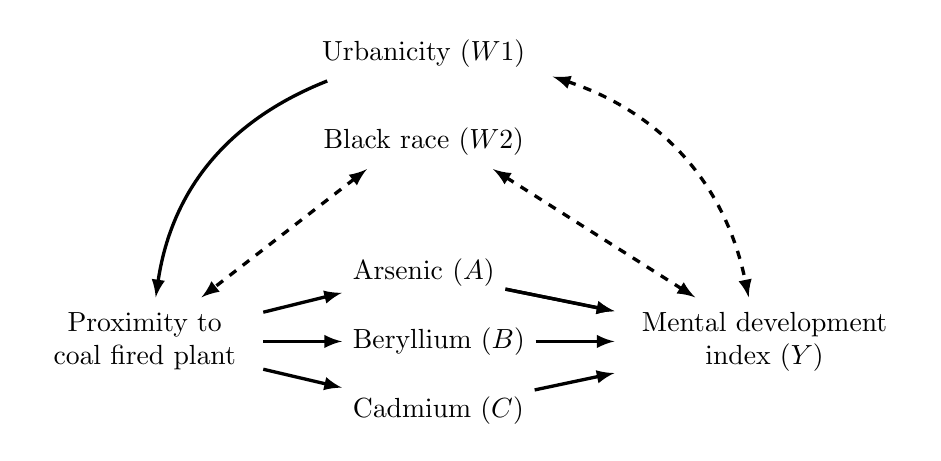
\begin{tikzpicture}[>=latex, line join=bevel, very thick]
	     %
             \node[](coal){\begin{tabular}{c}Proximity to \\ coal fired plant\end{tabular}};
             \node[above right=of coal, shift={(0,-1)}](a){Arsenic $(A)$};
             \node[right=of coal](b){Beryllium $(B)$};
             \node[below right=of coal, shift={(0,1)}](c){Cadmium $(C)$};
             \node[ right=of b] (y) {\begin{tabular}{c}Mental development\\ index $(Y)$\end{tabular}};
             \node[above =of a] (w1) {\begin{tabular}{c}\\Black race $(W2)$\end{tabular}};
             \node[above =of w1, shift={(0,-1)}] (w2) {\begin{tabular}{c}Urbanicity $(W1)$\end{tabular}};
             %
             \path[-latex] (coal) edge[] (a);  
             \path[-latex] (coal) edge[] (b);  
             \path[-latex] (coal) edge[] (c);  
             \path[-latex] (a) edge[] (y);  
             \path[-latex] (b) edge[] (y);  
             \path[-latex] (c) edge[] (y);  
             \path[-latex] (a) edge[] (y);  
             \path[latex-latex] (w1) edge[style=dashed] (y);  
             \path[latex-latex] (w1) edge[style=dashed] (coal);  
             \path[-latex] (w2) edge[bend right] (coal);  
             \path[latex-latex] (w2) edge[style=dashed, bend left] (y);  
          \end{tikzpicture} 
}
    \end{column}
  \end{columns}
\end{frame}


\begin{frame}{Motivating example: coal fired power plants and cognitive development}
(Possible) Causal questions of interest:
    \begin{description}
      \item[Causal independent exposure-response] How does the population average MDI change as we increase Arsenic but hold other exposures constant
      \item[Causal joint exposure-response] How does the population average MDI change as we increase all exposures by the same amount
      \item[Causal attributable difference] How does the population average MDI change after we eliminate all/some exposures?
      \item[Causal generalized impact difference] How does the population average MDI change after we reduce all/some exposures by some policy-relevant amount?
    \end{description}
\end{frame}


\begin{frame}{A note on study questions}
Causal inference allows us to ask questions with answers that make sense to people who don't know what regression is, without sacrificing rigor
\bigskip

I always encourage students to ask causal questions because it helps focus and choose methods even when causality is hopeless.

\end{frame}




%%%%%%%%%%%%%%%%%%%%%%%%%%%%%%%%
%:1 Counterfactuals and potential outcomes
%%%%%%%%%%%%%%%%%%%%%%%%%%%%%%%%
\title{}
\subtitle{Foundational concepts}
\author{
	\begin{itemize}
		\item Counterfactuals
		\item Potential outcomes and consistency
		\item Causal identification assumptions
	\end{itemize}
}
\date{}
\begin{frame}
	\titlepage
\end{frame}

\begin{frame}{Notation, notation notes}
	\begin{description}
		\item[Univariate exposure/treatment] $A$, with realized values $a$ (binary for now)
		\item[Univariate outcome] $Y$, $y$
		\item[Confounders] $\bm{W}$, $\bm{w}$
		\item[Non-confounding covariates] $\bm{V}$, $\bm{v}$
		\item[Individuals] Individuals will be noted with $i$ subscripts, as little as necessary (e.g. $y_{i}$)
		\item[Simplification] Except when necessary, I will introduce most concepts for time-fixed data
	\end{description}
\end{frame}



\begin{frame}[c]{Counterfactuals}
Counterfactuals refer to the \emph{policies} that are counterfactual for each individual: unseen dopplegangers that follow each policy of interest (here ``yes'' or ``no'' exposure)

		\begin{center}
			\begin{tabular}{lcccc}\hline
				id      & W   & A\footnote{Here, I distinguish between "setting" $A$ to some value via a policy versus "observing" $A$ at the same value.}   & Y   &  \\\hline
				1       & 2.9 & yes & no  & factual     \\
				$1_{y}$ & 2.9 & yes & ?   & counterfactual      \\
				$1_{n}$ & 2.9 & no  & ?   & counterfactual      \\
				2       & 0.5 & no  & yes & factual     \\
				$2_y$   & 0.5 & yes & ?   & counterfactual      \\
				$2_n$   & 0.5 & no  & ?   & counterfactual      \\
				\hline
			\end{tabular}
		\end{center}

\end{frame}

%\begin{frame}[c]{Closest possible worlds and counterfactuals}
%	\only<1>{For causal inference, we are often interested in the ``closest possible world'' to our own (we'd like to make inference relevant to our observed world, so we pick a counterfactual that is ``close'' to our own world).}
%	\only<2>{This can be actualized by filling in covariate values such that the counterfactual observations are identical to the observed data in all ways other than possibly the exposure and outcome
%	
%	\begin{center}
%	\begin{tabular}{lcccc}\hline
%id & W & A & Y & counterfactual\\\hline
%1& 2.9& yes & no & no\\
%$1^{yes}$ & \color{red}{2.9}& yes & ?& yes\\
%$1^{no}$& \color{red}{2.9}&  no & ?&  yes\\
%2& 0.5& no & yes& no\\
%$2^{yes}$ & \color{red}{0.5}& yes & ?& yes\\
%$2^{no}$ & \color{red}{0.5}&  no & ?& yes\\
%\hline
%\end{tabular}
%\end{center}
%}
%
%\end{frame}
\begin{frame}[c]{Potential outcomes}
	\only<1>{\textbf{Potential outcome}: $Y^a$, or the value\footnote{These are ``deterministic'' potential outcomes. We could similarly define ``stochastic'' potential outcomes via a probability distribution on $Y^a$.} of the outcome $Y$ we would have observed, had exposure been set to some value $a$}

	\only<2>{An individual (additive) causal effect of ``yes'' vs. ``no'' exposure is defined as $Y_i^{yes}-Y_i^{no}$.\footnote{In the potential outcomes framework, this is a way of saying ``no causation without manipulation'' - causal effects are undefined without hypothetical manipulation.} 
	
	\bigskip
	
	In this sense, \textbf{causal effects are defined without data}, so to learn anything about causal effects we need a way to link what we see (data and/or priors), with what could be (potential outcomes).}

\end{frame}

\begin{frame}[c]{Potential outcomes and causal consistency}
	\only<1>{The link from our factual world to counterfactual observations happens via \textbf{causal consistency}, which is that $Y_i^a = Y_i$ if $A_i=a$. That is, we would expect an individual to have identical outcomes if we set $A=a$ via policy or if we observed $A=a$.\footnote{There is a second assumption here that will be discussed later, which is included in the alternative stable unit treatment value assumption (SUTVA) that was originally used to link counterfactuals with observed data} }
	\only<2>{
		Given causal consistency, we can fill in some of the table
		\begin{center}
			\begin{tabular}{lcccc}\hline
				id        & W                  & A   & Y                &  \\\hline
				1         & 2.9                & yes & no               & factual     \\
				$1^{yes}$ & \color{black}{2.9} & yes & \color{red}{no}  & counterfactual      \\
				$1^{no}$  & \color{black}{2.9} & no  & ?                & counterfactual      \\
				2         & 0.5                & no  & yes              & factual     \\
				$2^{yes}$ & \color{black}{0.5} & yes & ?                & counterfactual      \\
				$2^{no}$  & \color{black}{0.5} & no  & \color{red}{yes} & counterfactual      \\
				\hline
			\end{tabular}
		\end{center}

	}
	\only<3>{
		Here's another way you may see it:\footnote{Rubin, D. B. (1974). Estimating causal effects of treatments in randomized and nonrandomized studies. Journal of Educational Psychology, 66(5), 688–701.}

		\begin{center}
			\begin{tabular}{lccccccc}\hline
				id & W   & A   & Y   & Y$^{yes}$       & Y$^{no}$         \\\hline
				1  & 2.9 & yes & no  & \color{red}{no} & ?                \\
				2  & 0.5 & no  & yes & ?               & \color{red}{yes} \\
				\hline
			\end{tabular}
		\end{center}
	}
\end{frame}


\begin{frame}[t]{The fundamental problem of causal inference}
	\visible<1->{

	Recall that we define an individual, additive\footnote{We could also use ratios and the relative scale.} causal effect as the difference  $Y_i^{yes}-Y_i^{no}$
	\begin{center}
		\begin{tabular}{lcccccccc}\hline
			id & W   & A   & Y   & Y$^{yes}$         & Y$^{no}$  & $Y^{yes}-Y^{no}$          \\\hline
			1  & 2.9 & yes & no  & \color{black}{no} & ?& ?                  \\
			2  & 0.5 & no  & yes & ?                 & \color{black}{yes} & ?\\
			\hline
		\end{tabular}
	\end{center}
	}
	\visible<2>{
		\bigskip

		Even with causal consistency, at least one of the potential outcomes necessary for defining a causal effect will always be missing. This is known as the \textbf{fundamental problem of causal inference}. To make progress we need more assumptions.}
\end{frame}


%\begin{frame}[t]{Aside: The fundamentaler problem of causal inference}
%	\visible<1->{
%		Edwards et al.\footnote{Edwards et al. (2000) \emph{IJE}} demonstrated that, due to measurement error $(W,A,Y)$ are not represented by observed quantities (we see mis-measured versions), so the problem is more accurately represented as
%		\begin{center}
%			\begin{tabular}{lccccccc}\hline
%				id & W & A & Y & Y$^{yes}$ & Y$^{no}$ \\\hline
%				1  & ? & ? & ? & ?         & ?        \\
%				2  & ? & ? & ? & ?         & ?        \\
%				\hline
%			\end{tabular}
%		\end{center}
%	}
%	\visible<2>{
%		\bigskip
%
%		We can't make any progress at all if we don't believe our data (or add assumptions). For today let's believe the data.
%	}
%\end{frame}


%%%%%%%%%%%%%%%%%%%%%%%%%%%%%%%%
%:2 Identification
%%%%%%%%%%%%%%%%%%%%%%%%%%%%%%%%

\begin{frame}[c]
	\frametitle{Individual and average causal effects}
	\visible<1->{Even if we can't estimate individual causal effects, we can use additional assumptions to estimate average potential outcomes ($E(Y^a|\bm{W}=\bm{w})$), and hence average causal effects:}
	\visible<1->{
		\begin{description}
			\item[Population/sample average causal effect ] $E(Y^a) - E(Y^{a^*}) = E(Y^a - Y^{a^*})$
			\item[ Average affect among the ``$a$-treated''  ] $E(Y^a - Y^{a^*} | A=a)$
			\item[ Causal dose-response ] $f(y^a)$
			\item[Conditional average causal effects ] $E(Y^a - Y^{a^*}|\bm{W}=\bm{w})$
		\end{description}
	}

\end{frame}
%
%\begin{frame}[c]{G-null hypothesis}
%One "universal" definition of a cause comes from the g-null hypothesis:
%
%\[
%E(Y^{a^*}) = E(Y^a)
%\]
%For all possible values of $a^*$, and $a$  
%
%\only<2> {Any violation of the g-null hypothesis for an exposure $A$ implies that $A$ is a cause of $Y$}
%\end{frame}


\begin{frame}[c]{Whose average?}
  \only<1>{The definition of a population average causal effect presupposes a specific population, often called the \textbf{target population}.}
  \only<2>{Defining the target population is essential to evaluating the utility of estimates of causal effects, and often necessitates concepts of \textbf{generalizability} or \textbf{transportability}\footnote{Ask Daniel Westreich: westreic@email.unc.edu}}
  \only<3>{Formally \textbf{generalizing} or \textbf{transporting} causal effects relies applying conditional average causal effects (conditional on $\bm{W}$ and/or $\bm{V}$) to populations with different distributions of $\bm{W}$ and/or $\bm{V}$ from the study sample.}
  \only<4>{$\bm{W}$ and $\bm{V}$ are sometimes referred to as the ``context", or ``state'', since they are often non-modifiable factors that can influence the effectiveness of a policy. We may think of factors like exposure susceptibility, race, and socioeconomic status as classical examples of factors that differ across populations and by which conditional causal effects may vary greatly.}
  \only<5>{The term ``average causal effect'' is thus vacuous without first defining the target population, which often is not the study population.}
\end{frame}




\begin{frame}[c]{Causal identification conditions
	\tiny{
		\only<4->{No interference}\only<6->{, conditional exchangeability}\only<8->{, positivity}
	}}
	\only<1>{Returning to the main thread, causal consistency alone is not sufficient to license the estimation of average causal effects.}
	\only<2>{Consider if $A$ is vaccination and $Y$ is SARS-COV-2 infection. Your infection, if not vaccinated ($Y^{no}$) doesn't just depend on your vaccination status, but also the vaccination status of your neighbor.}
	\only<3,4>{
	\visible<3,4>{If one's potential outcome depends also on others' exposure the potential outcome would have to be denoted by your exposure, as well as everyone else's exposure: (the hideous looking $Y^{a_i, \{a_j \in A: j \neq i\}}$).}
	\visible<4>{This makes the math much more difficult.\footnote{though causal inference is sometimes still possible: Hudgens et al (2008) \emph{J Am Stat Assoc}}
		Under the \textbf{no interference} assumption (based on subject matter knowledge), your potential outcomes don't depend on the exposures of others, so we are safe to just use simpler notation and math.}
		}
	\only<5>{\textbf{Causal consistency} and \textbf{no interference} give us "observed" potential outcomes, where we know your potential outcome under the exposure that you, in fact, received. However, recall that causal inference requires us to know something about the potential outcomes under counterfactual exposures/policies, as well.}
	\only<6>{
		The link to counterfactual policies is provided by \textbf{conditional exchangeability}\footnote{This is sometimes referred to as a ``no unmeasured confounding or selection bias'' assumption}, given by
		}
         \only<6,7>{
		$$
			Y^a \amalg A  | \textbf{W}= \textbf{w}
		$$
        }
	\only<6>{which reads as "The potential outcome under a given policy is independent of exposure, given confounders." This assumption means that, in a stratum of confounders $\bm{W}$, we can consider the "observed" potential outcomes to stand in for the "missing" potential outcomes because in that stratum the individuals are "exchangeable" with each other
	}
	\only<7>{This doesn't give us individual potential outcomes but we can "impute" average potential outcomes in strata of confounders via: 
	  $$
	      E(Y^a | A\neq a,  \textbf{W}= \textbf{w}) = E(Y^a | A= a,  \textbf{W}= \textbf{w})
	  $$
	  While not obvious, this has *almost* given us enough to estimate average potential outcomes for an entire population, and thus causal effects.
	}
	\only<8>{
		Notably, the conditional causal effect 
	       $$
	           E(Y^a | A= a,  \textbf{W}= \textbf{w})
	      $$
              only makes sense if it is \emph{possible} to observe the combination $A=a,  \textbf{W}= \textbf{w}$. One way to re-write this is:
		$$
			Pr(A=a | \textbf{W}= \textbf{w}) > 0
		$$
		for each policy $a$ being compared. This assumption is referred to as \textbf{positivity}.
	}
	\only<9>{
		\textbf{Aside:} Positivity means that, for a given policy $a$, that value of exposure must be \emph{possible} at all joint levels of confounders. \textbf{Sparsity}\footnote{this has been called "stochastic non-positivity"} can occur when $A=a$ is possible, but simply not observed in the data. Here's a distinction:
		    \begin{description}
      \item[Non-positivity] always biased, and our causal question may be ill-posed (e.g. effect of hysterectomies among people born without a uterus)
      \item[Sparsity] biased, but we may reduce/eliminate bias with more data or a model
    \end{description}
	}
	\only<10>{
		No interference, conditional exchangeability and, positivity are known as \emph{causal identification conditions} because they are sufficient to ``identify'' a causal effect from observed data.\footnote{but not necessarily the data in hand} In a perfectly run randomized trial, these conditions will hold by design. In observational studies, we must rely on subject matter knowledge to judge how well these assumptions are met.
	}
\end{frame}

\begin{frame}[c]{Conditional exchangeability and DAGs}
Conditional exchangeability can be (roughly) read off of a causal directed acyclic graph (DAG). These two tools inhabit different causal inference paradigms (potential outcomes versus do-calculus\footnote{Pearl, Judea. Causality. Cambridge University Press, 2009.}), but they are mathematically equivalent. For example, the following conditional exchangeability statement (among others) is consistent with the following DAG.
  \begin{columns}
    \begin{column}[c]{.5\textwidth}
 		\begin{align}
			MDI^{no~arsenic} \amalg Arsenic  | {Urbanicity}= {yes}\nonumber\\
		\end{align}
   \end{column}
    \begin{column}[c]{.5\textwidth}
	  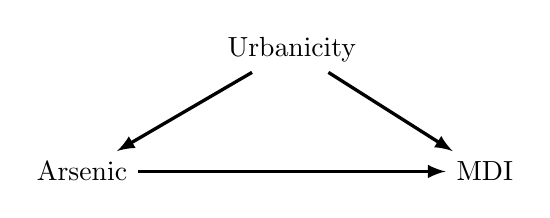
\begin{tikzpicture}[>=latex, line join=bevel, very thick]
	     %
             \node[](x){Arsenic};
             \node[above right=of x] (z) {Urbanicity};
             \node[below right=of z] (y) {MDI};
             %
             \path[-latex] (x) edge[] (y);  
             \path[-latex] (z) edge[] (x);  
             \path[-latex] (z) edge[] (y);  
          \end{tikzpicture} 

    \end{column}
  \end{columns}
This is another place where "subject matter knowledge" is essential for causal inference - if we don't know our DAG we can't assess causal assumptions. 

\end{frame}

\begin{frame}[c]{Minimal causal unit: conditional effects}
Together the causal identification conditions give us the following:

\[ E(Y^a | W=w) = E(Y | A=a, W=w) \]

Which we can read as: the average \emph{potential} outcome under the policy "Set A=a" in a group where $W=w$ is equal to the average \emph{observed} outcome in a subset of your data where $A=a$ and $W=w$

This link allows us to "see" causal effects in actual data. If we don't believe we can get a conditional effect somewhere, we generally can't do causal effect estimation.


\end{frame}


\begin{frame}[c]{So you are telling me we need to adjust for confounders?}
Potential outcomes/causal inference has been criticized for being a re-statement what we already know: we need to adjust for confounders.
\bigskip

While it's true that causal inference has formalized the definition of confounding (via DAGs)
\end{frame}


%\begin{frame}[c]{Time-varying data: causal identification conditions}
%	\only<1>{A remarkable achievement of Robins\footnote{Robins (1986) Math Mod} was generalizing causal identification conditions for causal effects of time-varying (longitudinal) exposures. This allows identification of causal effects of policies that are \textbf{static regimes} such as ``always exposed", ``never exposed'' or \textbf{dynamic regimes} such as``if $\bm{W_k}=\bm{w}$, then set $A_k=a$. Else $A_k=a^*$''\footnote{Regimes can ``deterministic'' like this or ``random,'' where values of $A_k$ are drawn from a distribution}
%	}
%	\only<2>{
%	    \textbf{No interference} in longitudinal data states that one's potential outcome at any time is independent of any exposure from any other individual at any time.\footnote{ Subject matter knowledge necessary here would not substantially differ from that required in the time-fixed setting.}
%	}
%
%	\only<3>{
%	    \textbf{Conditional exchangeability} in longitudinal data states that exposure at a given time (e.g. monthly exposure levels for silica workers) must be independent of future potential outcomes \emph{under a specific policy}, given past values of confounders, prior censoring\footnote{Late entry is never mentioned, but must also be considered when it occurs} and outcome history, and past values of exposure under the specific policy. \footnote{See Young et al (2011) \emph{Stat Biosci} for excellent formal representation}
%	    
%	    This may require additional subject matter knowledge relative to the time-fixed setting in that we should better understand joint predictors of censoring and the outcomes of interest.
%	}
%	\only<4>{
%	    \textbf{Positivity} in longitudinal data is also defined for time-specific exposures. The notable feature here is not that all levels of exposure must be possible at all strata of exposure, but that levels of exposure \emph{under the policy of interest} must be possible. This allows for causal inference in occupational data, where exposure may not occur off work, as long as the policy is a dynamic regime such as ``remain uncensored and, if at work, remain exposed below the exposure limit.''\footnote{See Young et al (2011) Stat Biosci for excellent formal representation}
%	}
%\end{frame}



%%%%%%%%%%%%%%%%%%%%%%%%%%%%%%%%
%:mixtures problems
%%%%%%%%%%%%%%%%%%%%%%%%%%%%%%%%
\title{}
\subtitle{Extending foundational concepts with our coal-fired power plant example}
\author{
	\begin{itemize}
		\item Why textbook examples fail mixtures
		\item Inverse probability weighting and G-computation
		\item Wrap-up
	\end{itemize}
}
\date{}
\begin{frame}
	\titlepage
\end{frame}


%%%%%%%%%%%%%%%%
\begin{frame}[t]
  \frametitle{Textbook examples fail us for mixtures}
Our textbook examples have only included on single binary exposure $A$. 

\bigskip
But mixtures have continuous, and potentially highly exposures, so we'll almost always have sparsity where certain ranges of exposure just are not observed for different covariate/exposure strata.

\bigskip
And a mixture of multiple exposures (Arsenic, Beryllium, Cadmium) means we can't rely (without modification) on the wealth of methods for single exposures. 

%\bigskip
%Mixtures also often bring up issues of environmental justice (e.g. historical exposure inequity due to racism) 

\end{frame}



\begin{frame}[t]
We'll investigate these issues without resorting to (too much) notation. Recall our (simulated) example 
{\footnotesize
	  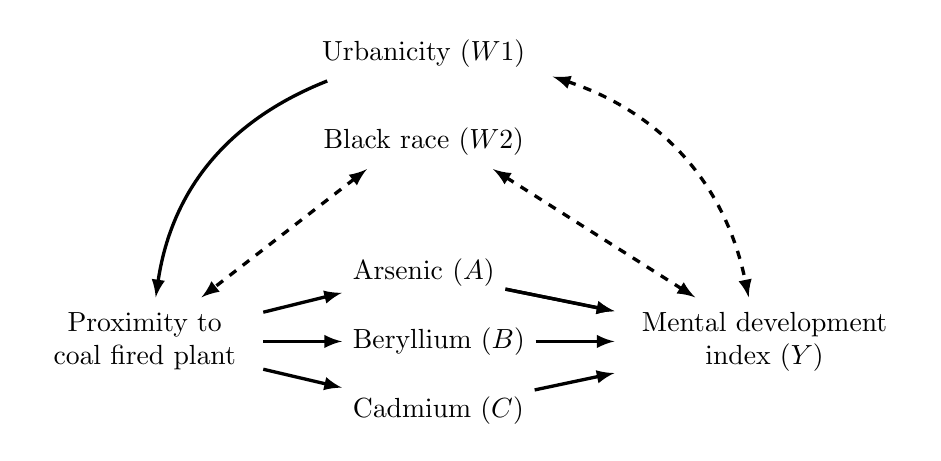
\begin{tikzpicture}[>=latex, line join=bevel, very thick]
	     %
             \node[](coal){\begin{tabular}{c}Proximity to \\ coal fired plant\end{tabular}};
             \node[above right=of coal, shift={(0,-1)}](a){Arsenic $(A)$};
             \node[right=of coal](b){Beryllium $(B)$};
             \node[below right=of coal, shift={(0,1)}](c){Cadmium $(C)$};
             \node[ right=of b] (y) {\begin{tabular}{c}Mental development\\ index $(Y)$\end{tabular}};
             \node[above =of a] (w1) {\begin{tabular}{c}\\Black race $(W2)$\end{tabular}};
             \node[above =of w1, shift={(0,-1)}] (w2) {\begin{tabular}{c}Urbanicity $(W1)$\end{tabular}};
             %
             \path[-latex] (coal) edge[] (a);  
             \path[-latex] (coal) edge[] (b);  
             \path[-latex] (coal) edge[] (c);  
             \path[-latex] (a) edge[] (y);  
             \path[-latex] (b) edge[] (y);  
             \path[-latex] (c) edge[] (y);  
             \path[-latex] (a) edge[] (y);  
             \path[latex-latex] (w1) edge[style=dashed] (y);  
             \path[latex-latex] (w1) edge[style=dashed] (coal);  
             \path[-latex] (w2) edge[bend right] (coal);  
             \path[latex-latex] (w2) edge[style=dashed, bend left] (y);  
          \end{tikzpicture} 
}
\end{frame}

\begin{frame}[t]{Basics of the data}
    \begin{columns}
    \begin{column}[t]{.6\textwidth}
    The first 5 observations
	  % Table generated by Excel2LaTeX from sheet 'Sheet1'
\begin{tabular}{rrrrrr}\hline
\multicolumn{1}{l}{urbanicity} & \multicolumn{1}{l}{black} & \multicolumn{1}{l}{as} & \multicolumn{1}{l}{be} & \multicolumn{1}{l}{cd} & \multicolumn{1}{l}{mdi} \\\hline
1     & 0     & 0.814 & 0.931 & 1.64  & 82.5 \\
0     & 0     & 0.243 & 0.354 & 0.243 & 93.9 \\
1     & 0     & 0.404 & 0.406 & 0.665 & 123 \\
0     & 1     & 0.366 & 0.241 & 0.218 & 115 \\
1     & 0     & 0.245 & 0.347 & 0.335 & 110 \\\hline
\end{tabular}%
    \end{column}
    \begin{column}[t]{.4\textwidth}
    Pearson correlation matrix
	  % Table generated by Excel2LaTeX from sheet 'Sheet2'
\begin{tabular}{l|r|r|r|}
\multicolumn{1}{r}{} & \multicolumn{1}{l}{as} & \multicolumn{1}{l}{be} & \multicolumn{1}{l}{cd} \bigstrut[b]\\
\cline{2-4}as    & 1     &   &  \bigstrut\\
\cline{2-4}be    & 0.86  & 1     &  \bigstrut\\
\cline{2-4}cd    & 0.76  & 0.68  & 1 \bigstrut\\
\cline{2-4}\end{tabular}%
    
    \end{column}
  \end{columns}
  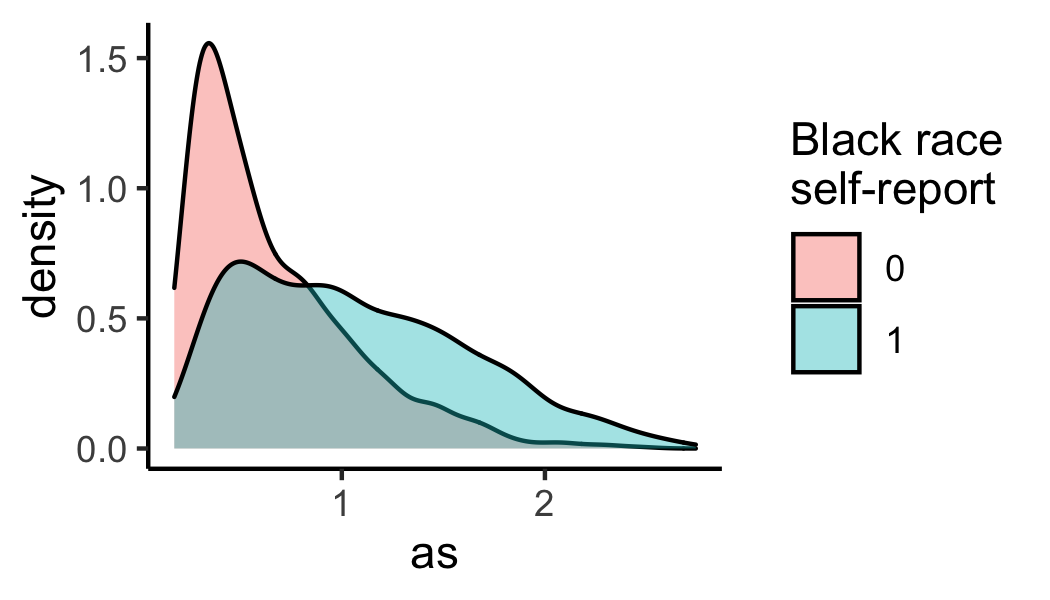
\includegraphics[height=.15\textwidth]{../analyses/output/as_dens.png}%
  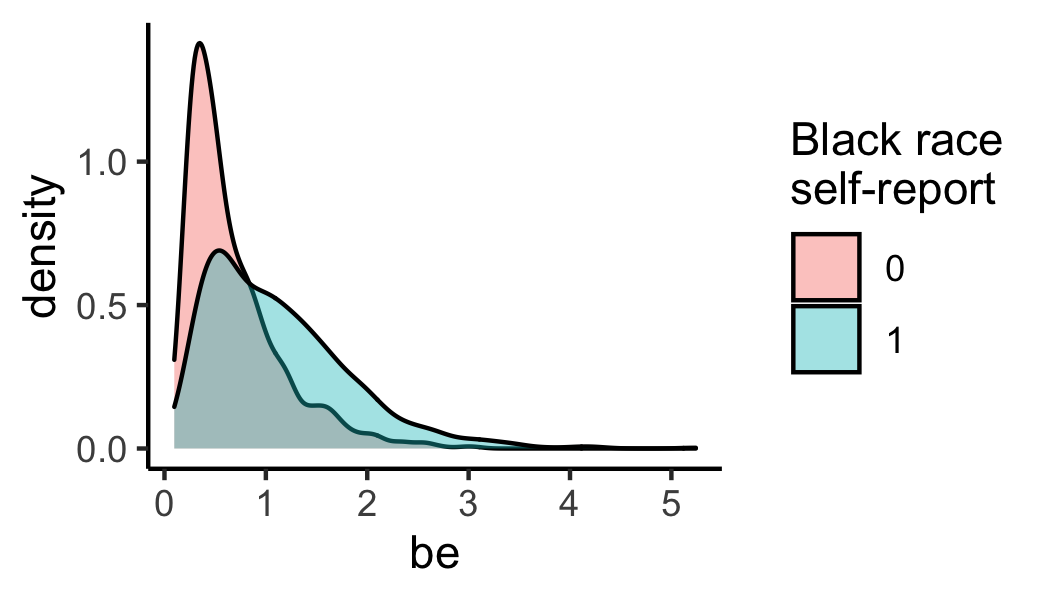
\includegraphics[height=.15\textwidth]{../analyses/output/be_dens.png}%
  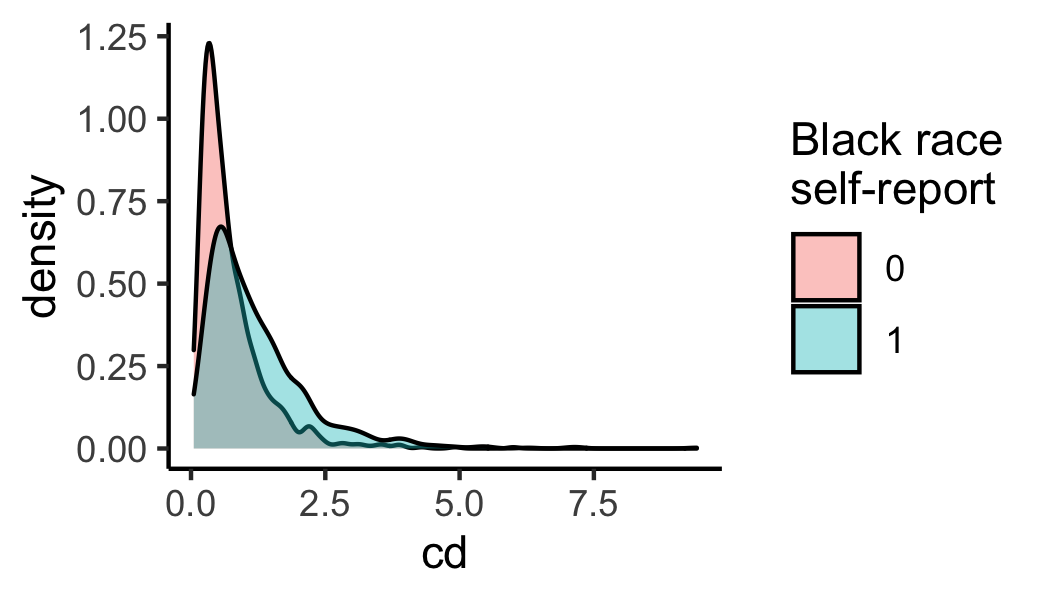
\includegraphics[height=.15\textwidth]{../analyses/output/cd_dens.png}%
  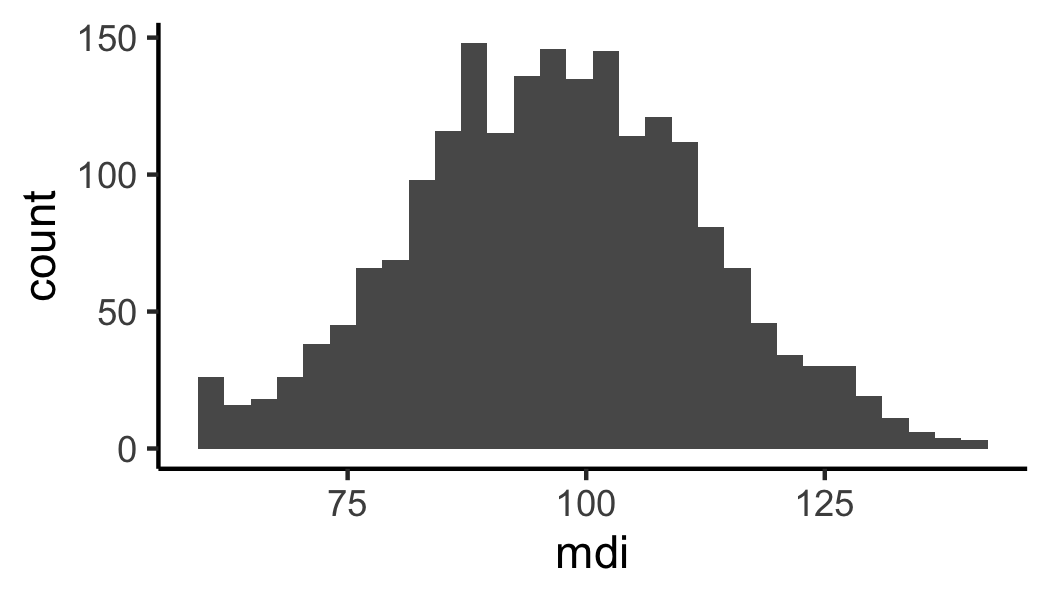
\includegraphics[height=.15\textwidth]{../analyses/output/mdi_dens.png}
\end{frame}


\begin{frame}[t]{Textbook examples and continuous exposures}
Under our DAG, for a single exposure (say arsenic), the "minimal causal unit" that we need is:
$$
E(MDI | A=a, B=b, C=c, Confounders)
$$
Roughly, to identify a causal effect of increasing arsenic by 1 unit (e.g. an independent causal dose response), we would need to observe, roughly, that at all values of the other exposures and confounders, we see some variation in arsenic of about 1 unit.\footnote{Sort of, this is language for discrete variables, which is fuzzy to apply here but to be more exact requires measure theory :(}
\end{frame}



\begin{frame}[t]{Textbook examples and continuous exposures}
 
   \begin{columns}
    \begin{column}[c]{.5\textwidth}
     \only<1>{Visually, we can see whether sparsity is an issue (it is, and we've known it for a long time)\footnotemark}
     \only<2>{
       Here we can see that a one unit change (1.5 $\rightarrow$ 2.5) in arsenic is possible and (informally) identified when Beryllium = 1.0 ug/m$^3$
       \bigskip
       
       "Identification" here just informally means that we have some data points on both the left and right sides of the red bar, where the MDI for those individuals would be used in estimating the causal contrast (very roughly speaking)
       
     }
     \only<3>{It may be possible (positivity) but it is not observed (sparsity) when Beryllium = 3.0 ug/m$^3$}
     \only<4>{This issue is well described and it seems hopeless that we'll be biased.}
     \only<5>{However, note that, a 1 unit change  (2.5 $\rightarrow$ 3.5) in arsenic is observed  when Beryllium = 3.0 ug/m$^3$}
     \only<6>{If we can assume that the rate of change (e.g. regression coefficient) of the outcome is modeled accurately within the range of the data, then the effect of  As = 1.5 $\rightarrow$ As = 2.5, is "parametrically" identified.
     \bigskip
     
     A statistical model allows us to share information to estimate valid causal effects where we have no data, \emph{provided the model is correct}. This is dangerous and difficult to diagnose, but (caveat emptor) it's possible.
     }
     \only<7>{The amount of extrapolation and reliance on assuming a correct model grows very quickly as we condition on more and more exposures/confounders, which is part of the \textbf{curse of dimensionality} }
    \end{column}
    \begin{column}[c]{.5\textwidth}
    \begin{figure}
		 \only<1>{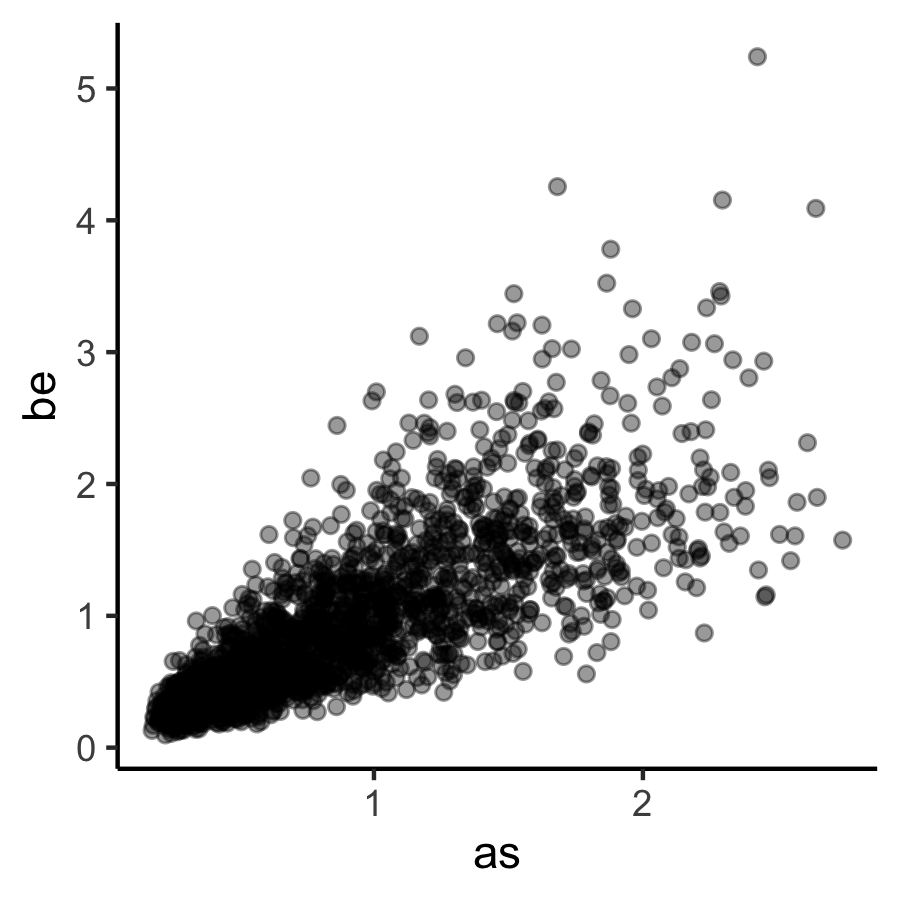
\includegraphics[height=.8\textheight]{../analyses/output/as_be_scatter.png}}%
		 \only<2>{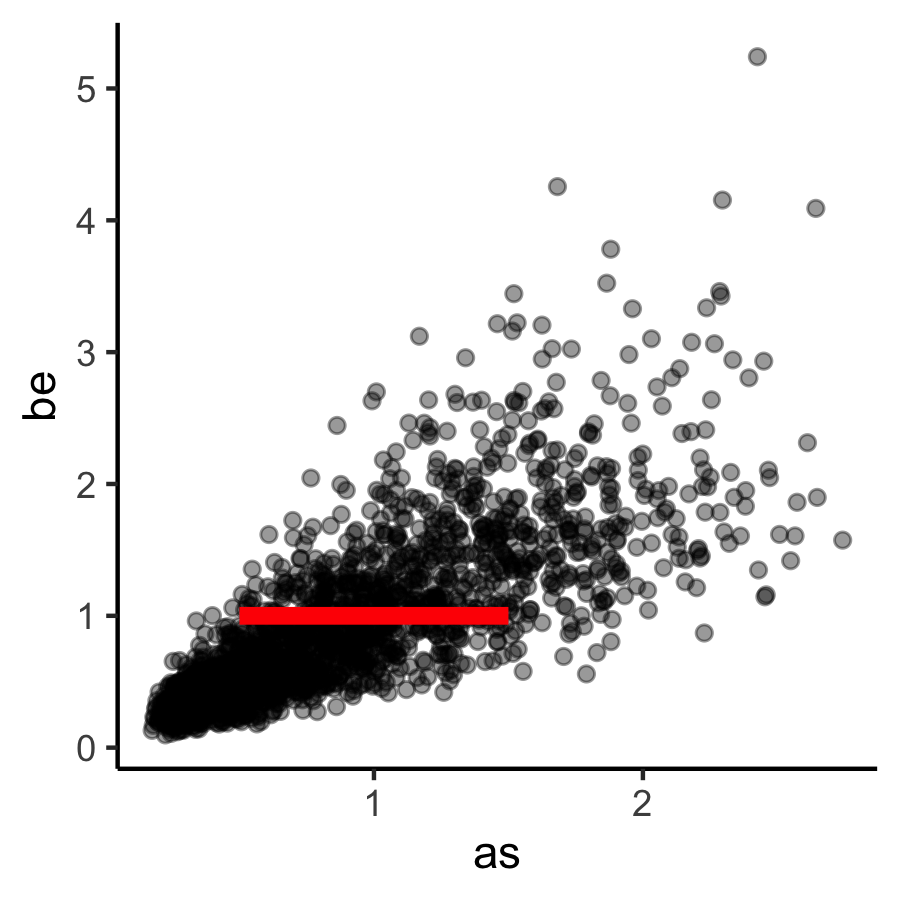
\includegraphics[height=.8\textheight]{../analyses/output/as_be_scatter_b1.png}}%
		 \only<3,4>{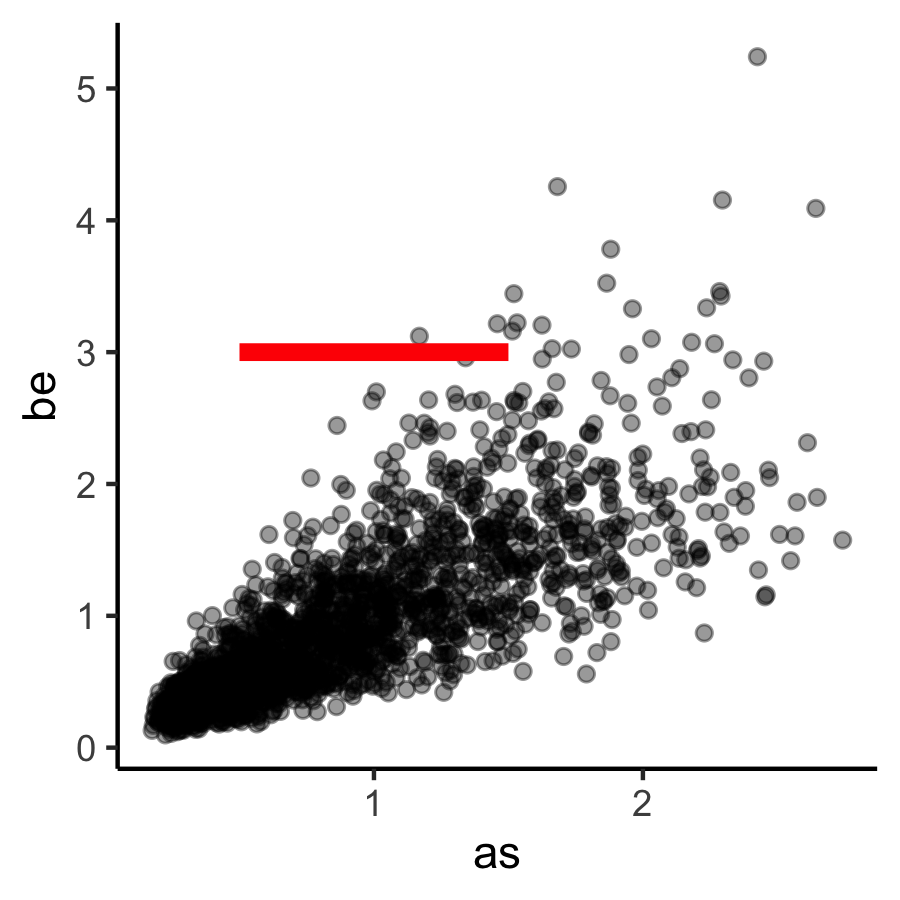
\includegraphics[height=.8\textheight]{../analyses/output/as_be_scatter_b2.png}}%
		 \only<5>{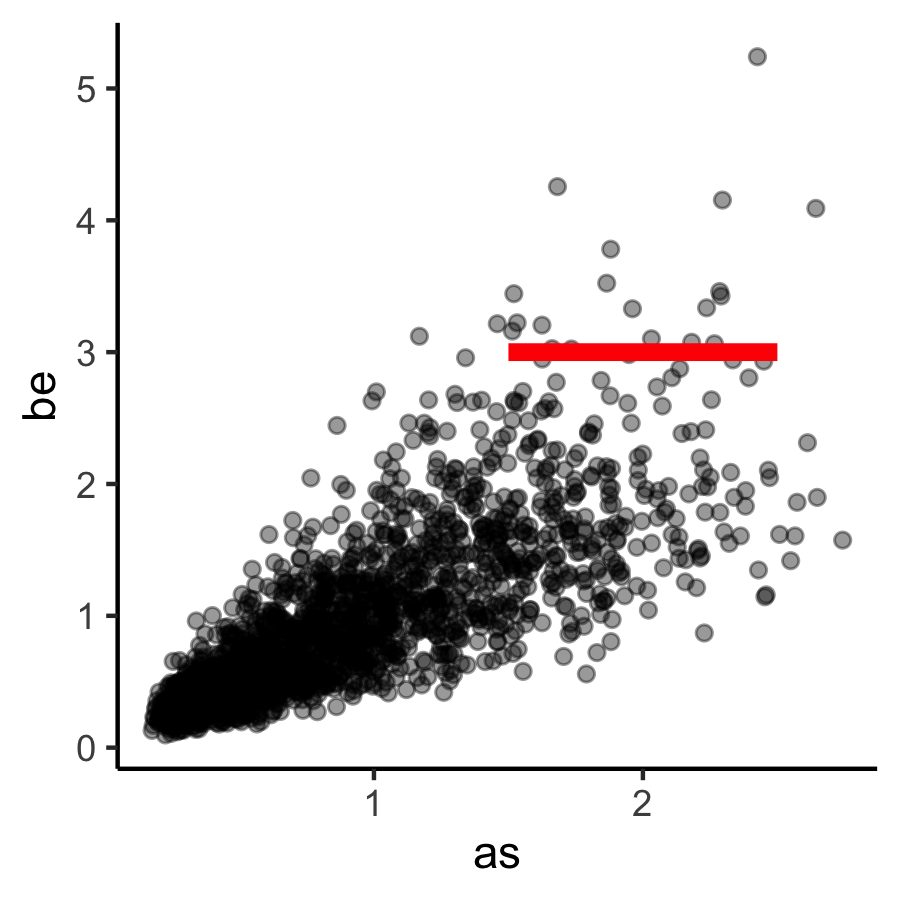
\includegraphics[height=.8\textheight]{../analyses/output/as_be_scatter_b3.png}}%
		 \only<6->{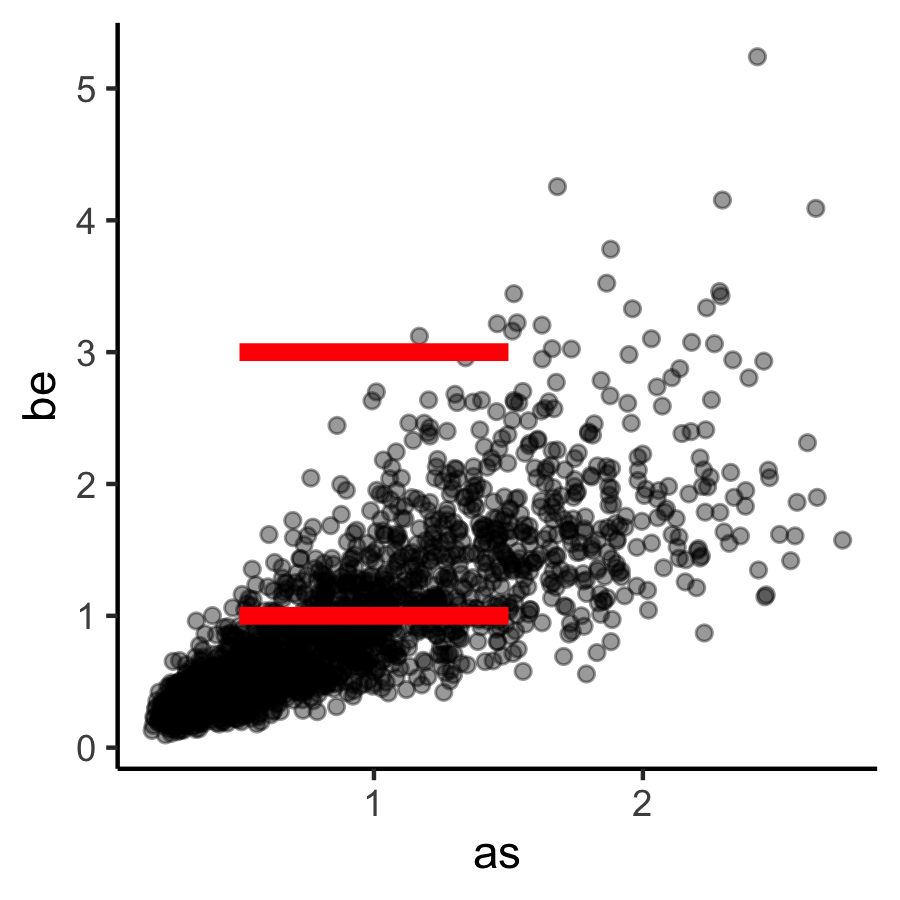
\includegraphics[height=.8\textheight]{../analyses/output/as_be_scatter_b4.png}}%
   \end{figure}
   \end{column}
  \end{columns}
 \only<1>{ \footnotetext{Snowden, et al. Framing air pollution epidemiology in terms of population interventions, with applications to multi-pollutant modeling. Epidemiology 26.2 (2015): 271.}}
\end{frame}

\begin{frame}[t]{Continuous exposures beyond textbook examples}
The curse of dimensionality is part of the \textbf{fundamental problem of mixtures}: correlation between components of a mixture means we should suspect co-pollutant confounding, but adjusting for that confounding in statistical models can lead to problems on its own. To address this information problem, causal inference in mixtures can potentially benefit from: 
\bigskip

    \begin{itemize}
      \item Dimension reduction (PCA, clustering, profile regression)
      \item Shrinkage, selection, Bayesian priors (LASSO, E-net, Bayesian regression/selection, other regularized machine learning)
      \item {\only<2>{\color{red}}Changing the question} (WQS, Bayesian kernel machine regression, quantile g-computation)
    \end{itemize}


\end{frame}


\begin{frame}[t]{Textbook examples and multiple exposures} 
  \begin{columns}
    \begin{column}[c]{.5\textwidth}
	    \only<1>{Textbook examples of causal inference rarely mention more than one exposure}
	    \only<2>{The fundamental problem of mixtures really describes problems with estimating the effect of one exposure, holding others constant: }
   	    \only<3>{Alternatively, consider the effect of two exposures, where the contrast is again roughly a comparison of the average outcomes at each end of the red line:  }
   	    \only<4>{Here we transform exposure so that "1 unit" of exposure is "1 quantile" (e.g. a quartile length)}
   	    \only<5->{This effect is occasionally discussed in the textbook examples as a "joint effect"
	    \bigskip
             
             see e.g. VanderWeele, T. J. (2009). On the distinction between interaction and effect modification. Epidemiology, 20(6), 863-871.}
    \end{column}
    \begin{column}[c]{.5\textwidth}
    		 \only<1>{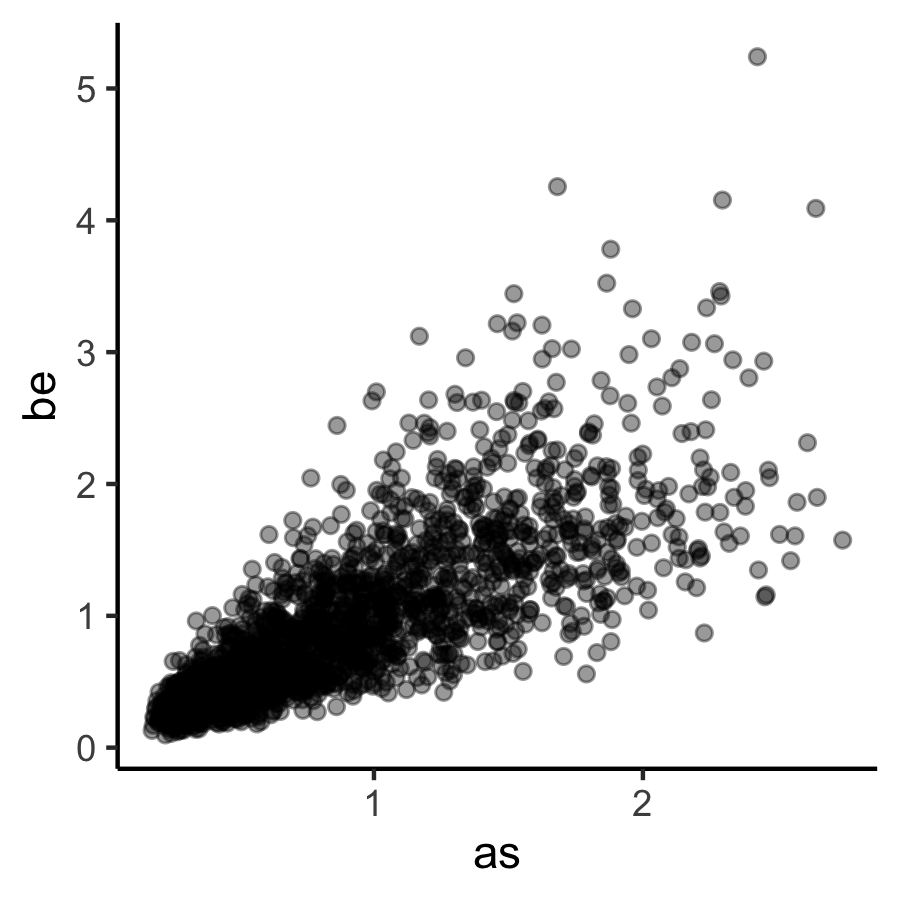
\includegraphics[height=.8\textheight]{../analyses/output/as_be_scatter.png}}%
    		 \only<2>{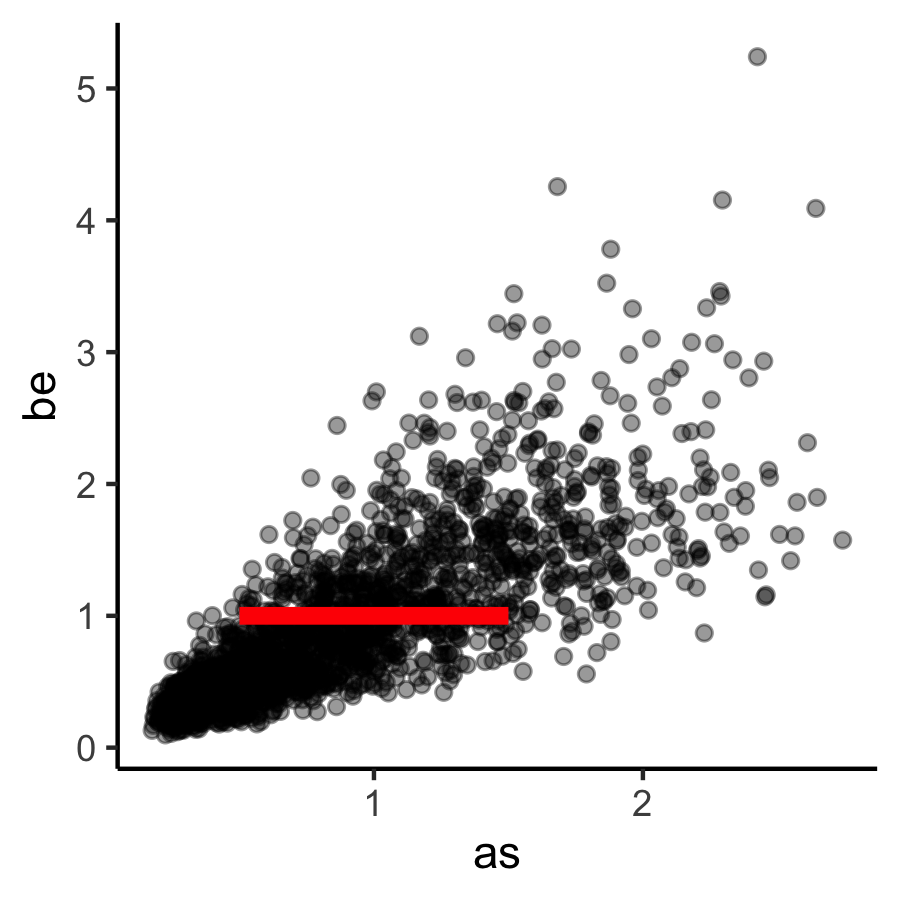
\includegraphics[height=.8\textheight]{../analyses/output/as_be_scatter_b1.png} $$E(y^{a+1}|b=1) - E(y^{a}|b=1)$$}%
    		 \only<3>{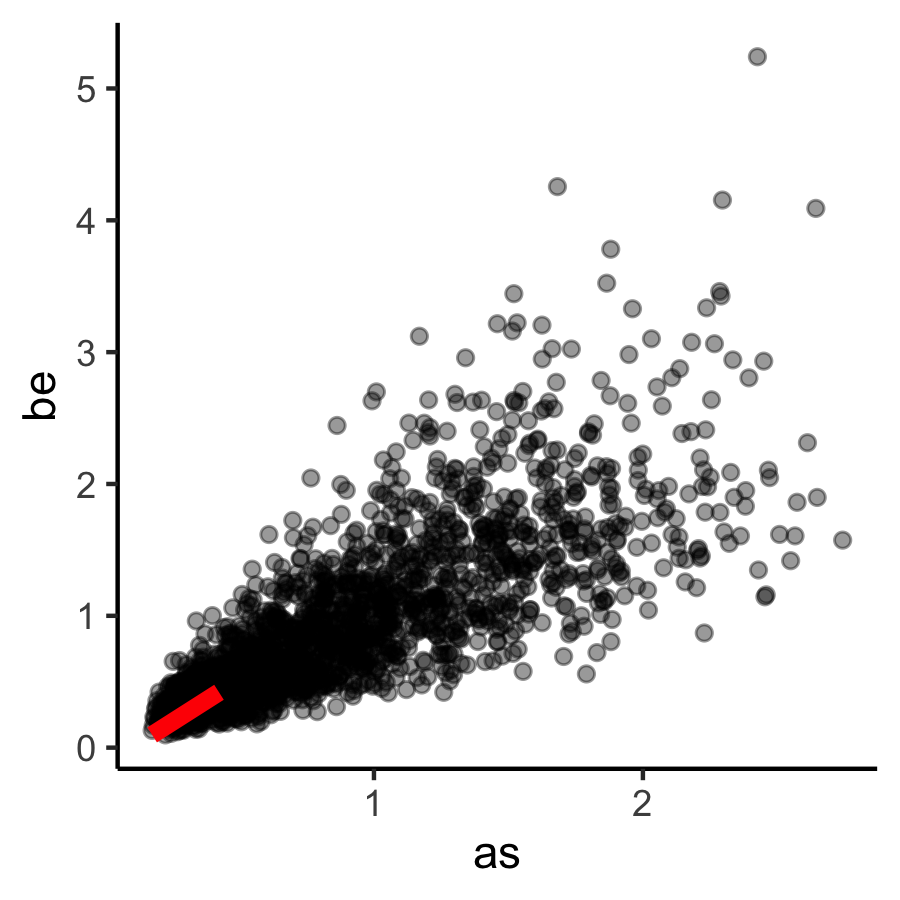
\includegraphics[height=.8\textheight]{../analyses/output/as_be_scatter_j1.png} $$E(y^{a+1, b+1}) - E(y^{a,b})$$}%
    		 \only<4>{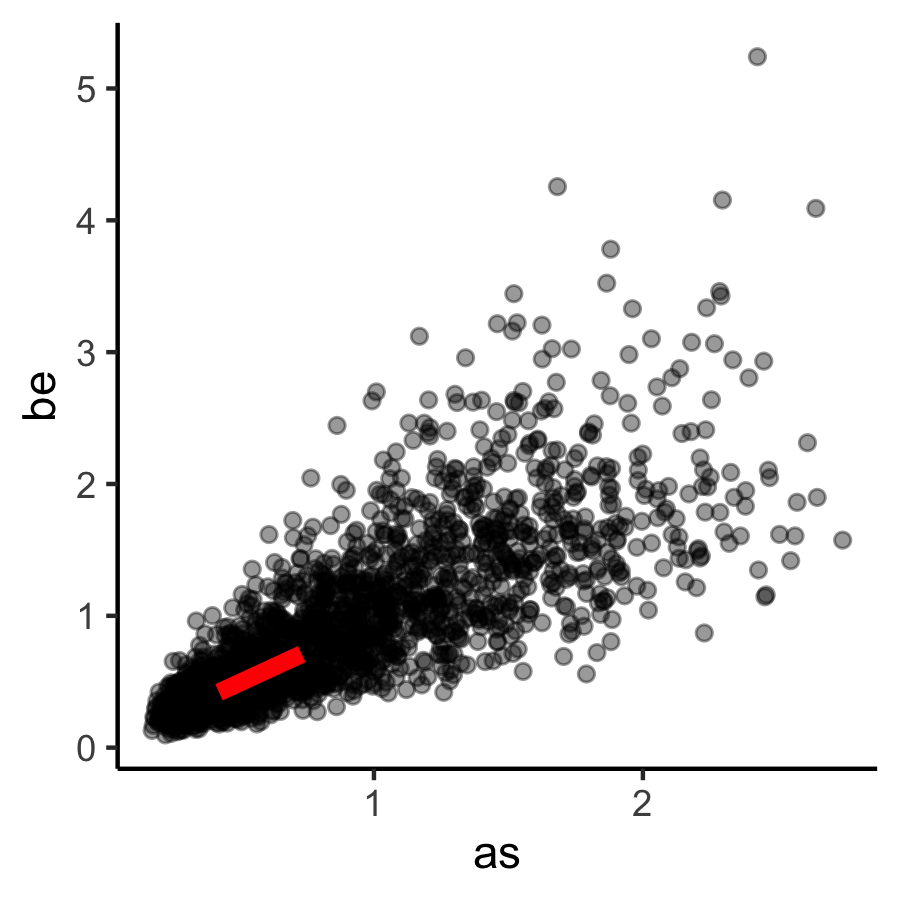
\includegraphics[height=.8\textheight]{../analyses/output/as_be_scatter_j2.png} $$E(y^{a+2, b+2}) - E(y^{a+1,b+1})$$}%
    		 \only<5>{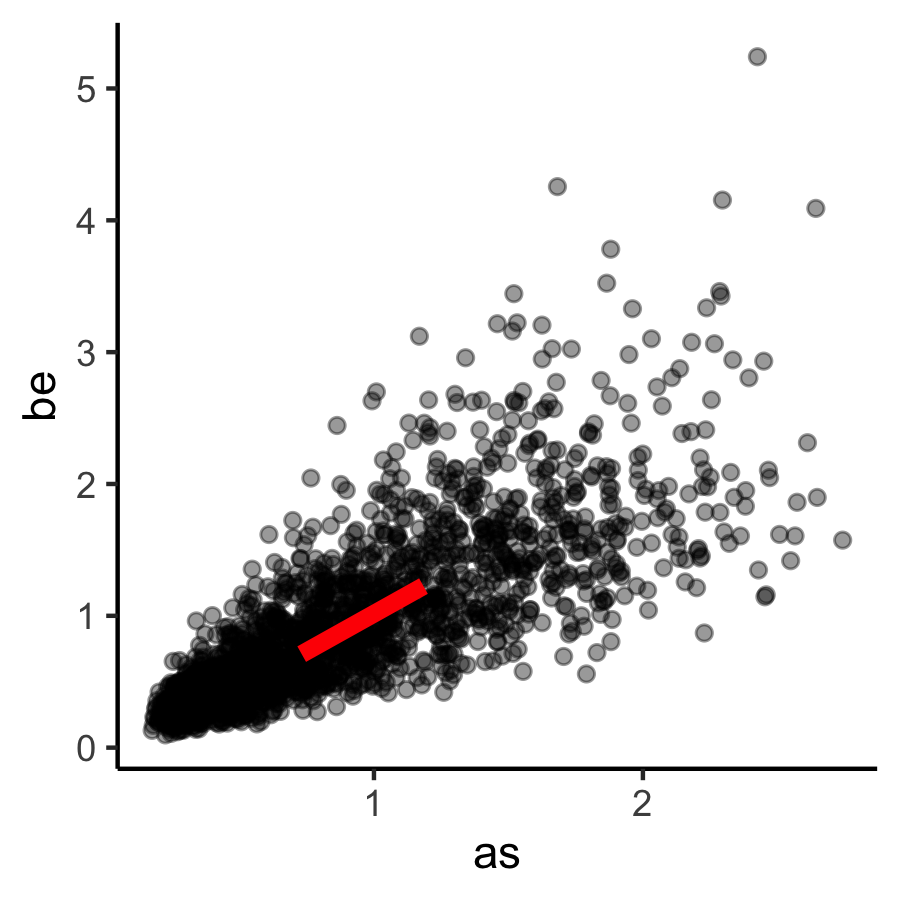
\includegraphics[height=.8\textheight]{../analyses/output/as_be_scatter_j3.png}$$E(y^{a+3, b+3}) - E(y^{a+2,b+2})$$}%
    		 \only<6>{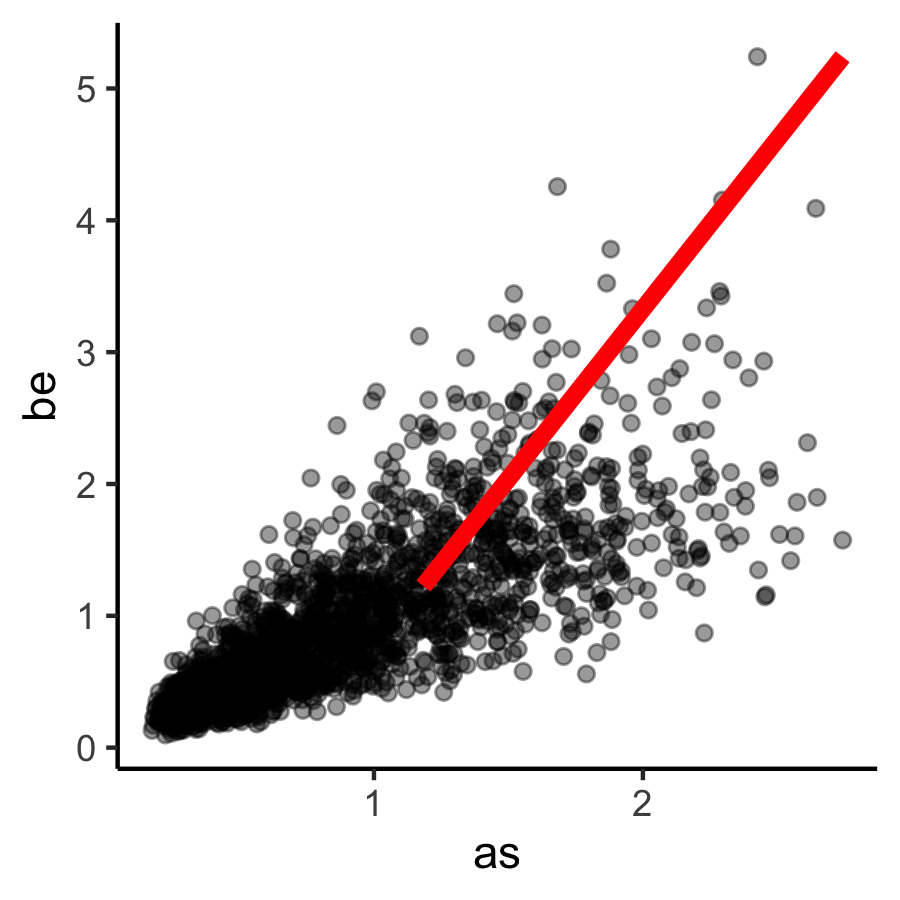
\includegraphics[height=.8\textheight]{../analyses/output/as_be_scatter_j4.png}$$E(y^{a+4, b+4}) - E(y^{a+3,b+3})$$}%
    \end{column}
  \end{columns}
\end{frame}


\begin{frame}[t]{Multiple exposures and marginal structural models}
    	  \begin{columns}
    \begin{column}[c]{.5\textwidth}
      \only<1-2>{
        Estimating a series of effects where we make comparisons of the average MDI at the right and left sides of the red line is roughly equivalent to turning our exposures into indicator variables
      }
      \only<3>{
        Here we see how the average MDI changes as we increase both arsenic and beryllium by one quantile at a time. 
                \bigskip
                
        (note that MDI was not on our scatter plot before)
      }
      \only<4>{
        If causal identification conditions are met (substituting our rough "model" for positivity/sparsity), then this can be interpreted as a regression line for a \textbf{marginal structural model}, which is just a model for average potential outcomes $E(y^{a,b}$)

      }
      \only<5->{
        Methods like Bayesian kernel machine regression\footnotemark{} and quantile g-computation\footnotemark{} \emph{can} give estimates from a \textbf{marginal structural model}. Quantile g-computation actually fits a model where we assume a parametric marginal structural model, giving a smooth regression line, possibly with a polynomial curve.

      }
    \end{column}
    \begin{column}[c]{.5\textwidth}
        		 \only<1>{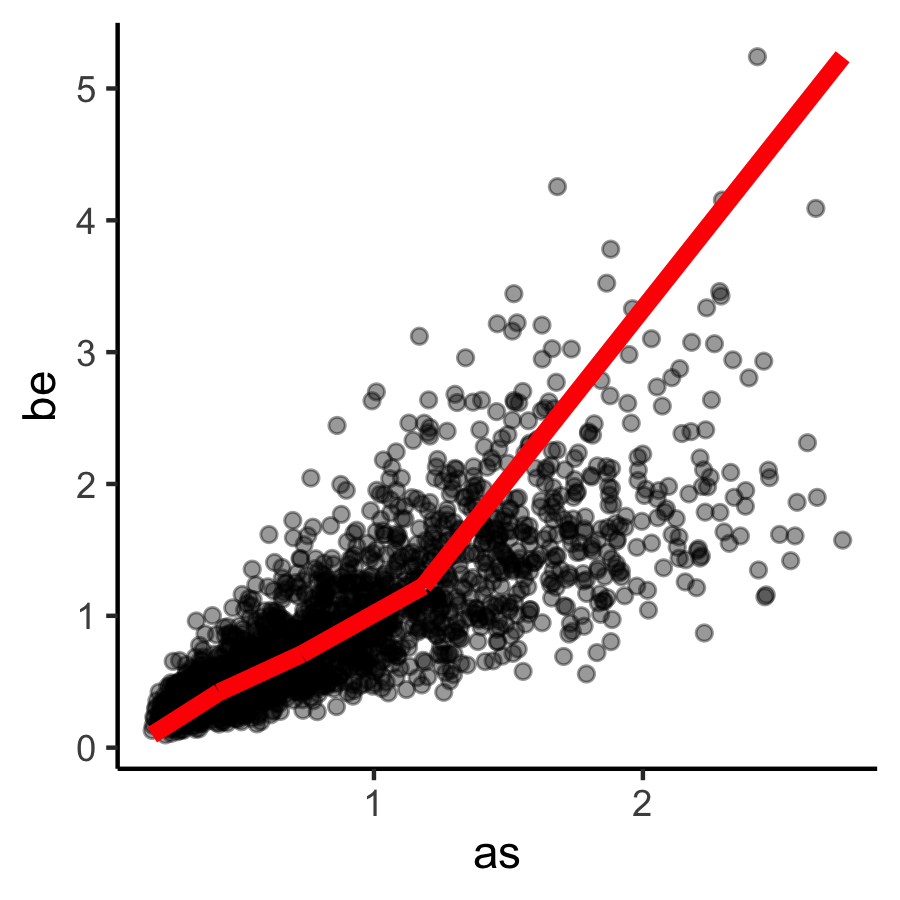
\includegraphics[height=.8\textheight]{../analyses/output/as_be_scatter_j5.png}}%
        		 \only<2-4>{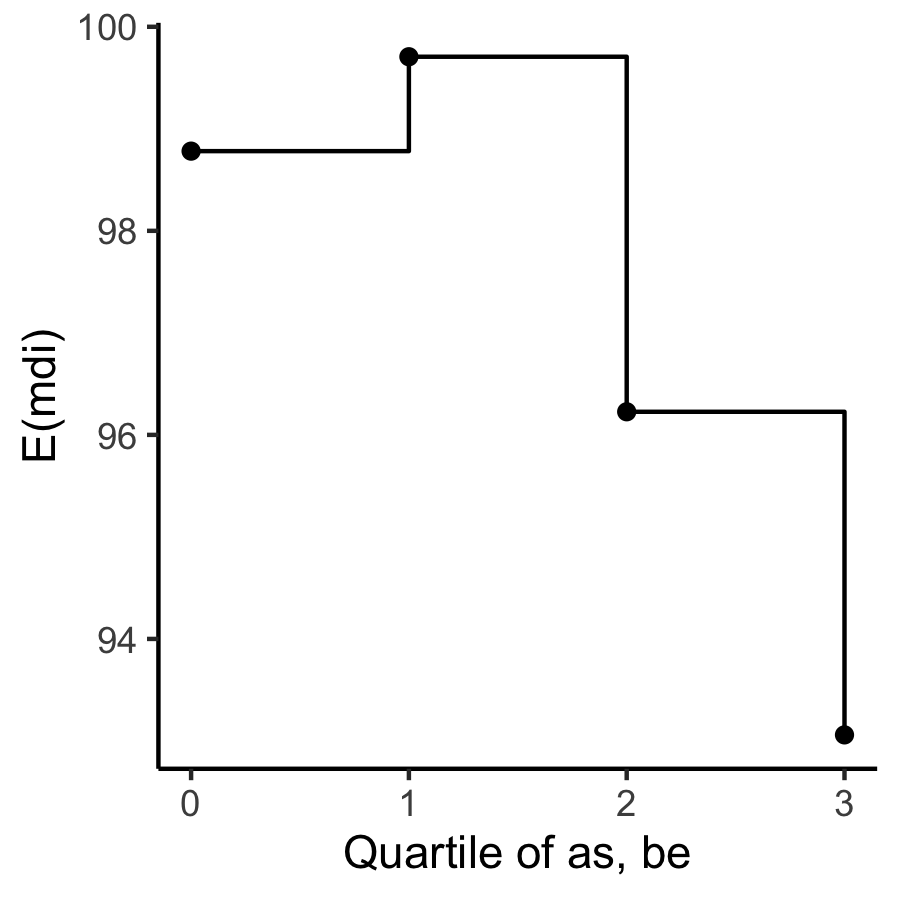
\includegraphics[height=.8\textheight]{../analyses/output/as_be_regline_1.png}}%
        		 \only<5>{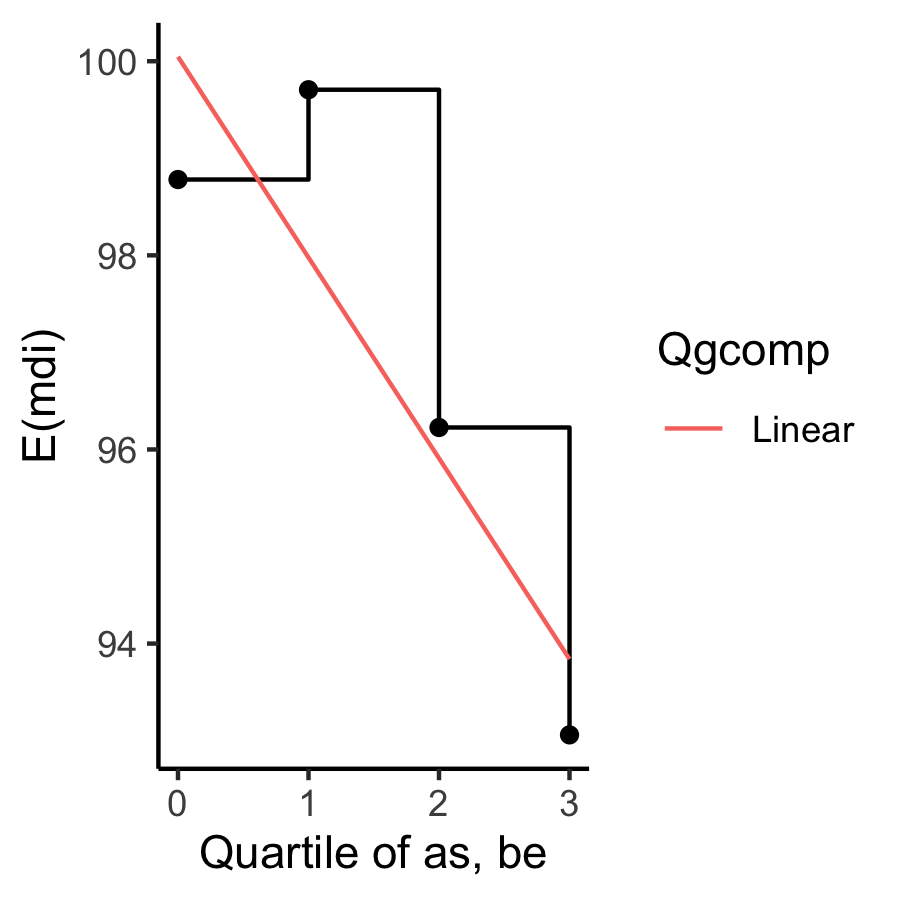
\includegraphics[height=.8\textheight]{../analyses/output/as_be_regline_qgc1.png}}%
        		 \only<6>{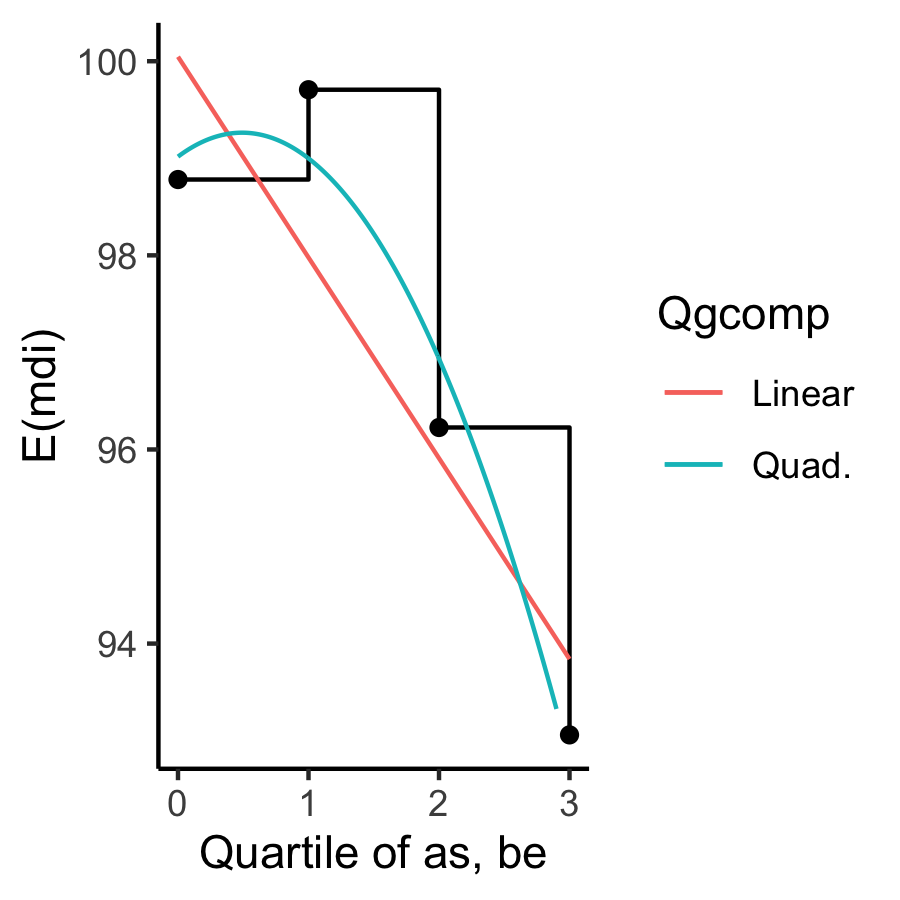
\includegraphics[height=.8\textheight]{../analyses/output/as_be_regline_qgc2.png}}%
    \end{column}
  \end{columns}

      \only<5->{
      \footnotetext[15]{\tiny Bobb, Jennifer F., et al. (2015) Bayesian kernel machine regression for estimating the health effects of multi-pollutant mixtures. Biostatistics 16(3), 493-508.}
      \footnotetext{\tiny Keil, A. P. et al (2020). A quantile-based g-computation approach to addressing the effects of exposure mixtures. Environmental health perspectives, 128(4), 047004.}}
\end{frame}

\begin{frame}[t]{Joint effects and the fundamental problem of mixtures}
  \begin{columns}
    \begin{column}[c]{.5\textwidth}
    One consequence of the fundamental problem of mixtures is that estimates of independent effects of a given exposure (here $\beta_1$) lose precision as correlation $\uparrow$
    \bigskip
    
    In contrast, marginal structural parameters for the joint effects of multiple exposures (here $\psi$) can \emph{gain} precision\footnotemark
     \bigskip
    
   Estimating joint effects may sometimes be a more efficient use of data than estimating independent effects in search of bad actors 
    \end{column}
    \begin{column}[c]{.5\textwidth}
    \begin{figure}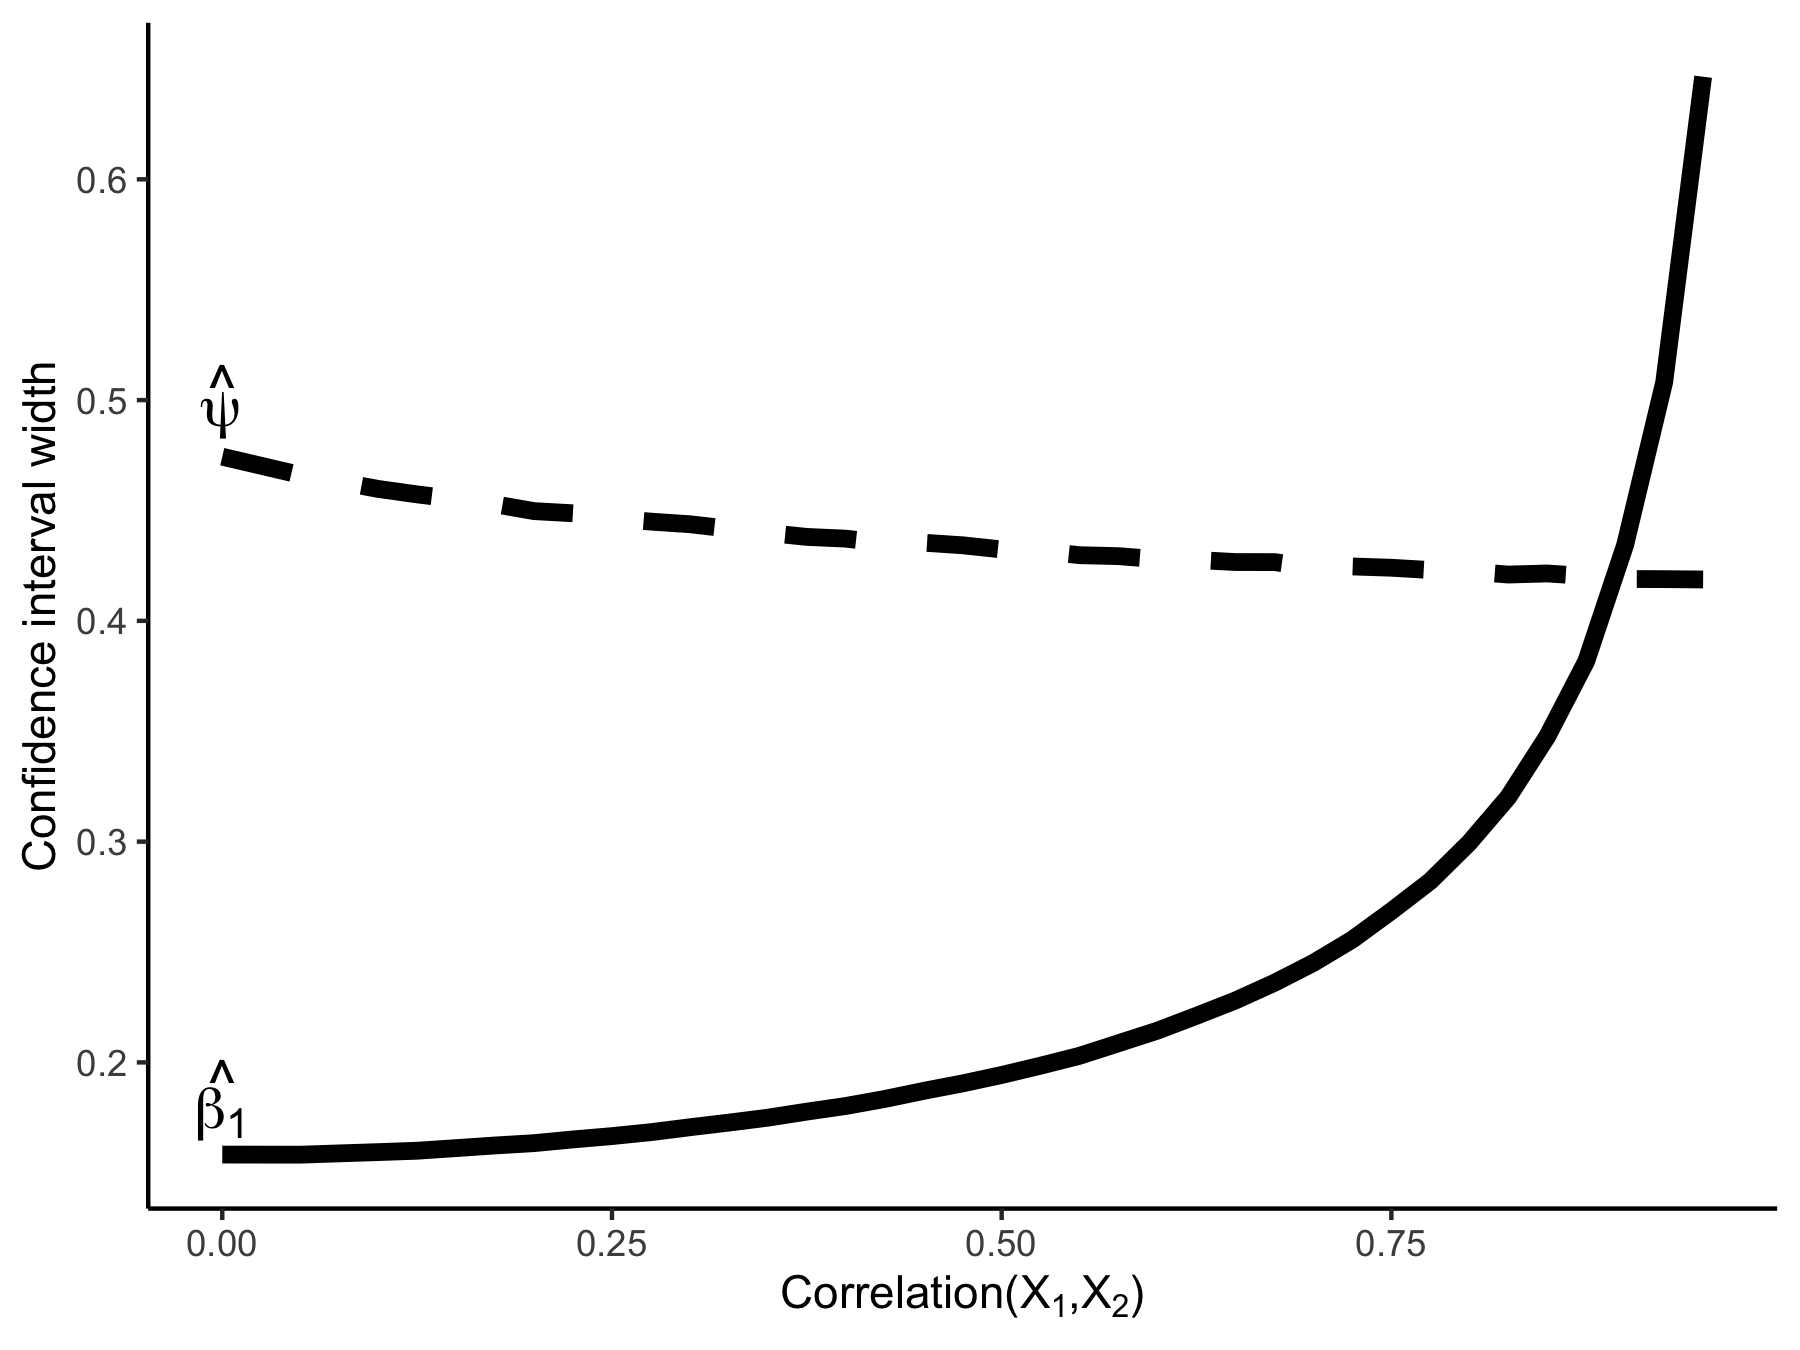
\includegraphics[width=\textwidth]{img/afig1_rev1.png}\end{figure}
    \end{column}
  \end{columns}
\footnotetext{\tiny Keil, A. P. et al (2020). A quantile-based g-computation approach to addressing the effects of exposure mixtures. Environmental health perspectives, 128(4), 047004.}



\end{frame}


%%%%%%%%%%%%%%%%
%\begin{frame}[t]{Textbook examples and continuous exposures}
%	\only<1>{
%	Recall how we represented potential outcomes with 2 new data colums for binary exposures:
%			\begin{center}
%			\begin{tabular}{lccccccc}\hline
%				id & W   & A   & Y   & Y$^{yes}$ & Y$^{no}$ \\\hline
%				1  & 2.9 & yes & no  & no         & ?        \\
%				2  & 0.5 & no  & yes & ?         & yes        \\
%				\hline
%			\end{tabular}
%		\end{center}
%	}
%	%
%	\only<2>{
%	Now consider a continuous exposure (e.g.A= $\mu$g/m$^3$ of airborne arsenic) that could take on many possible values
%	\begin{center}
%		\begin{tabular}{lccccccc}\hline
%			id & W   & A   & Y   & Y$^{-\infty}$         & Y$^{\infty}$           \\\hline
%			1  & 2.9 & 0.30 & no  & ? & ?                  \\
%			2  & 0.5 & 0.87  & yes & ?                 & ? \\
%			\hline
%		\end{tabular}
%	\end{center}
%	}
%	%
%	\only<3>{
%	We can again fill in some outcomes
%	\begin{center}
%		\begin{tabular}{lccccccc}\hline
%			id & W   & A  & Y   & Y$^{0.30}$         & Y$^{0.87}$           \\\hline
%			1  & 2.9 & 0.30 & no  & no & ?                  \\
%			2  & 0.5 & 0.87  & yes & ?                 & yes \\
%			\hline
%		\end{tabular}
%	\end{center}
%	}
%	%
%	\only<4>{
%	But what about other possible values of exposure?
%	\begin{center}
%		\begin{tabular}{lccccccccc}\hline
%			id & W   & A  & Y   & Y$^{0.30}$         & Y$^{0.87}$  & Y$^{1.0}$ & Y$^{3.1}$           \\\hline
%			1  & 2.9 & 0.30 & no  & no & ?& ?& ?                  \\
%			2  & 0.5 & 0.87  & yes & ?                 & yes & ?& ?\\
%			\hline
%		\end{tabular}
%	\end{center}
%	}
%	\only<5->{
%	But what about other possible values of exposure?
%	\begin{center}
%		\begin{tabular}{lcccccccccc}\hline
%			id & W   & A  & Y   & Y$^{0.0}$ & \ldots & Y$^{0.30}$  & \ldots & Y$^{0.87}$& \ldots   & Y$^{\infty}$           \\\hline
%			1  & 2.9 & 0.30 & no  & ?& \ldots& no &\ldots& ?&\ldots& ?                  \\
%			2  & 0.5 & 0.87  & yes & ?& \ldots& ?&\ldots                 & yes & \ldots& ?\\
%			\hline
%		\end{tabular}
%	\end{center}
%		\bigskip
%		
%		\visible<6>{
%		With binary exposures, we typically observe lots of individuals with $A=1$ and $A=0$ in the observed data, so we have some hope that the sparsity is not an issue (e.g. estimated $Pr(A=a) > 0$ at all levels of confounders, akin to positivity) and we can \emph{estimate} a causal effect.
%		\bigskip
%		
%		For continuous exposures, sparsity is guaranteed so the usual tools just do not seem to apply to these settings.
%		}
%	}
%
%\end{frame}

%%%%%%%%%%%%%%%%%%%%%%%%%%%%%%%%
%:5 worked example
%%%%%%%%%%%%%%%%%%%%%%%%%%%%%%%%
\section{Inverse probability weighting and g-computation to estimate joint and independent effects}
%%%%%%%%%%%%%%%%
\begin{frame}[t]
  \frametitle{Inverse probability weighting and marginal structural models}
   \only<1>{
    Inverse probability (of exposure) weighting (IPW) is a method for fitting marginal structural models or estimating other "policy" effects such as "how would the average outcome change if we reduced everyone's exposure to zero".
    \bigskip
    
    IPW within the mixtures context would rely on having a regression model for each exposure of interest, given confounders and co-exposures, and either an outcome model or a set of individuals who are "representative" of the policy contrast of interest
    \bigskip
    
    The basic idea is that the weighted population represents the original study population, had exposures been randomized
    }
    \only<2>{
    Methods for weighting with a single continuous exposure are well known, but typically work only in simple examples\footnote{Naimi, Ashley I., et al. Constructing inverse probability weights for continuous exposures: a comparison of methods. Epidemiology (2014): 292-299.;
    Kennedy, Edward H., et al. Nonparametric methods for doubly robust estimation of continuous treatment effects. JRSS. Series B, 79(4) (2017): 1229.
    }
    \bigskip
    
    For joint effects, one would need a model for each exposure of interest\footnote{Hernán, Miguel A., et al. Marginal structural models to estimate the joint causal effect of nonrandomized treatments. JASA 96.454 (2001): 440-448.}
    \bigskip
    
    I cannot recommend use of IPW in the mixtures context for estimating joint or independent effects and do not foresee a way in which current methods could be improved to change this
    }
\end{frame}
%%%%%%%%%%%%%%%%


\begin{frame}[t]
  \frametitle{g-computation}
    \only<1>{
    G-computation is a generalization of standardization and can be used for fitting marginal structural models or estimating other "policy" effects such as "how would the average outcome change if we reduced everyone's exposure to zero".
    \bigskip
    
    For time-fixed exposures, g-computation only requires a standard regression model \footnote{Snowden, Jonathan M et al. (2011) Implementation of G-computation on a simulated data set: demonstration of a causal inference technique. AJE 173(7): 731-738.}. Quantile g-computation is a special case.
    \bigskip
    
    G-computation extends to time-varying exposures, but requires more modeling\footnote{e.g. Keil, Alexander P., et al. (2014) The parametric G-formula for time-to-event data: towards intuition with a worked example. Epidemiology 25(6): 889.}
    }
    \only<2>{
    Basic g-computation in the coal plant data:
    
    \begin{enumerate}
      \item Fit a model for E(mdi | a, b, c, confounders)
      \item Make predictions from that model under the "policy" levels of exposure
      \item Contrast average predictions for the population or subgroups
    \end{enumerate}

     }
\end{frame}


\begin{frame}[t, fragile]
  \frametitle{g-computation}
  Step 1: fit a model
\begin{lstlisting}[language=R]
mdimod <- glm(mdi ~ as*urbanicity + 
  be*urbanicity + cd*urbanicity + 
  as*black + be*black + cd*black + 
  as*be + as*cd + be*cd, data=coalplant)
\end{lstlisting}
  Step 2: make predictions from that model (e.g. all exposures equal to 1.0)
\begin{lstlisting}[language=R]
preddata <- coalplant
preddata$as  <- median(coalplant$as)
preddata$be <- median(coalplant$be)
preddata$cd <- median(coalplant$cd)
preddata$pred_med <- predict(mdimod, newdata = preddata)
\end{lstlisting}
\end{frame}


\begin{frame}[t]
  \frametitle{g-computation}
Step 2: (continued)
% Table generated by Excel2LaTeX from sheet 'Sheet3'
\begin{tabular}{rrrrrrr}
\hline
\multicolumn{1}{l}{urbanicity} & \multicolumn{1}{l}{black} & \multicolumn{1}{l}{as} & \multicolumn{1}{l}{be} & \multicolumn{1}{l}{cd} & \multicolumn{1}{l}{mdi} & \multicolumn{1}{l}{pred\_med} \bigstrut\\
\hline
1     & 0     & 0.731 & 0.709 & 0.708 & 82.5  & 98.1 \bigstrut[t]\\
0     & 0     & 0.731 & 0.709 & 0.708 & 93.9  & 97.2 \\
1     & 0     & 0.731 & 0.709 & 0.708 & 123   & 98.1 \\
0     & 1     & 0.731 & 0.709 & 0.708 & 115   & 97.5 \\
1     & 0     & 0.731 & 0.709 & 0.708 & 110   & 98.1 \bigstrut[b]\\
\hline
\end{tabular}%
Here are the first 5 observations with predictions. The predictions represent the expected outcome (MDI) for someone with specific exposure/covariate values
\end{frame}

\begin{frame}[t, fragile]
  \frametitle{g-computation}
Step 3: Contrast average predictions for the population or subgroups
\begin{lstlisting}[language=R]
mean(preddata$pred_med)
mean(coalplant$mdi)
\end{lstlisting}
Taking the mean prediction over the population is, technically, "standardizing" to the empirical distribution of covariates in the data, and yields predicted MDI = 97.7, which is higher than the average observed MDI of 96.9. 
\bigskip

The population average MDI is, technically speaking, the expected MDI under the policy "do nothing." So we could contrast that with our expected MDI under the policy "set all exposures to the observed medians" and get an average MDI difference of 0.8, meaning we would expect the population average MDI to increase by 0.8 if we changed everyone's exposures to the median.
\end{frame}

\begin{frame}[t, fragile]
  \frametitle{g-computation}
Step 3: Contrast average predictions for the population or subgroups
\begin{lstlisting}[language=R]
mean(filter(preddata, black==1)$pred_med)
mean(filter(preddata, black==1)$mdi)
\end{lstlisting}
This same contrast among those in the population who self-identified as Black yields an estimate of 1.8. Ignoring uncertainty, this is a larger impact than is observed in the overall population suggesting effect measure modification for the policy effect. 
\end{frame}


\begin{frame}[t, fragile]
  \frametitle{g-computation interpretation}
If our causal identification conditions hold, and the linear model we fit is correct, then causal inference tells us that we can interpret our results causally.
\bigskip

This should not be the default - the hard work of causal inference is showing that the identification conditions hold at least approximately.
\bigskip

Without these conditions, g-computation still gives us a standardized effect estimate, which is as valid as any other estimate and has the advantage of directly targeting a scientific question of interest, rather than forcing a question that is answered by regression coefficients.
\end{frame}


\begin{frame}[t, fragile]
  \frametitle{g-computation: the "underlying fit"}
    \begin{columns}
    \begin{column}[c]{.4\textwidth}
    The "underlying fit" for g-computation could be anything, but I (didactically) opted for flexibility by including 9 product terms. (In practice, I use model fit criteria and model dx).
    \bigskip
    
    Product terms are difficult to interpret in this context, but note no strong evidence of EMM by race. 
    \end{column}
    \begin{column}[c]{.6\textwidth}
    {\scriptsize % Table generated by Excel2LaTeX from sheet 'Sheet4'
\begin{tabular}{l|rrrr}
\hline
\multicolumn{1}{r}{} & \multicolumn{1}{l}{Estimate} & \multicolumn{1}{l}{Std. Error} & \multicolumn{1}{l}{t-statistic} & \multicolumn{1}{l}{p-value} \bigstrut\\
\hline
(Intercept) & 100.32 & 1.44  & 69.46 & \multicolumn{1}{l}{<2e-16} \bigstrut[t]\\
as    & -2.59 & 2.87  & -0.90 & 0.37 \\
urbanicity & -0.56 & 1.33  & -0.43 & 0.67 \\
be    & -1.49 & 2.38  & -0.63 & 0.53 \\
cd    & -0.90 & 1.64  & -0.55 & 0.58 \\
black & 2.77  & 1.51  & 1.83  & 0.07 \\
as:urbanicity & -3.31 & 2.36  & -1.40 & 0.16 \\
urbanicity:be & 4.61  & 1.81  & 2.54  & 0.01 \\
urbanicity:cd & 0.96  & 1.06  & 0.91  & 0.37 \\
as:black & -0.72 & 2.64  & -0.27 & 0.78 \\
be:black & -2.15 & 2.09  & -1.03 & 0.30 \\
cd:black & -0.4999 & 1.2559 & -0.398 & 0.6907 \\
as:be & 0.6607 & 1.3525 & 0.489 & 0.6252 \\
as:cd & 0.3268 & 1.1621 & 0.281 & 0.7786 \\
be:cd & -0.1557 & 0.9339 & -0.167 & 0.8676 \bigstrut[b]\\
\hline
\end{tabular}%
}
    \end{column}
  \end{columns}
\end{frame}

\begin{frame}[t, fragile]
  \frametitle{g-computation: change in average MDI}
Using the same underlying model, I estimated more contrasts:
    \begin{itemize}
      \item The independent effects of reducing each exposure to zero (Attributable difference)
      \item The joint effect of "coal plant decommissioning" by cutting every individual's exposure according to the proportion we would expect based on local coal-plant emissions (96\% As, 91\% Be, 50\% Cd)\footnote{These are actually based on estimates for Milwaukee County from the 2014 National Emissions Inventory and used in a forthcoming publication: Keil, A. P., et al. (2021). Bayesian G-Computation to Estimate Impacts of Interventions on Exposure Mixtures: Demonstration with Metals from Coal-Fired Power Plants and Birth- weight. AJE}, versus no action (Generalized impact difference)     
     \item Both of the above restricted to Black participants only 
    \end{itemize}
 \end{frame}

\begin{frame}[t, fragile]
  \frametitle{g-computation: extending effect estimates}
  % Table generated by Excel2LaTeX from sheet 'Sheet5'
\begin{tabular}{rccccc}
\hline
      & \textbf{Everyone} &       & \textbf{Black} &       & \textbf{Non-Black} \bigstrut\\
\hline
\multicolumn{1}{l}{\textbf{Attr. mean diff.}} &       &       &       &       &  \bigstrut[t]\\
As & 2.80 (0.8,4.81)$^*$ &       & 3.42 (0.35,6.49) &       & 2.18 (-0.61,4.96) \\
Be & 0.23 (-1.43,1.9) &       & 1.28 (-0.97,3.52) &       & -0.82 (-3.03,1.38) \\
Cd & 0.58 (-0.5,1.65) &       & 0.94 (-0.62,2.5) &       & 0.21 (-1.22,1.63) \\
\multicolumn{1}{l}{\textbf{Joint effect}} &       &       &       &       &  \\
Shutdown & 3.89 (1.81,5.96) &       & 5.91 (2.91,8.90) &       & 1.84 (-0.09,3.76) \bigstrut[b]\\
\hline
\multicolumn{6}{l}{Positive values indicate exposure harmful/policy beneficial}\\
\multicolumn{6}{l}{$^*$Confidence intervals given in parentheses from bootstrapping (see code)}
\end{tabular}%
 \end{frame}

\begin{frame}[t, fragile]
  \frametitle{g-computation: interpretation}
  Under the causal identification conditions, correct model specification, eliminating arsenic exposure would result in a 2.8 point gain in the population average MDI, an effect which would be stronger among Black participants in the study (3.42).
  \bigskip
  
  Provided that we have accurately predicted what would happen to these exposures if local coal-fired power plants were shut down, then Black participants could have experienced a nearly 6 point gain in MDI.
  \bigskip
  
  Notably, the underlying model had only weak evidence for effect measure modification by race: these estimates also reflect the fact that Black participants were exposed to higher levels of exposure.
 \end{frame}

\begin{frame}[t, fragile]
  \frametitle{quantile g-computation: a special case}
  Recall that outcome regression potentially involves a lot of extrapolation for independent effects. Our "joint effect" of a shutdown may similarly involve (to a lesser extent) extrapolation because not all exposures were reduced by similar amounts.
  
  \bigskip
  I re-examined the data using quantile g-computation via the qgcomp R-package with a linear underlying model, and stratified by race. 
  
  \bigskip
  Quantile g-computation estimates a marginal structural model for a 1-quantile (default: quartile) increase in exposure.

 \end{frame}

\begin{frame}[t, fragile]
  \frametitle{quantile g-computation: a special case}
  % Table generated by Excel2LaTeX from sheet 'Sheet6'
\begin{table}
\begin{tabular}{lc}\hline
      & \textbf{Effect estimate} \\
      & \textbf{(95\% CI)} \\\hline
\textbf{Everyone} & -1.86 (-2.59,-1.14) \\
\textbf{Black} & -2.71 (-3.69,-1.74) \\
\textbf{Non-black} & -0.92 (-1.85,0.01) \\\hline
\end{tabular}

Note here that a negative value indicates exposure is harmful
\end{table}

 \end{frame}


\begin{frame}[t, fragile]
  \frametitle{Wrapping up}
    \begin{itemize}
      \item The hard work of causal inference is in the assumptions: one should take great care
      \item In our example, it's likely that other pollutants from coal-fired power-plants would affect MDI, so in real examples this simple analysis would be confounded
      \item In more complex scenarios, we may have modeling problems that require Bayesian solutions to reduce mean-squared error\footnote{This is relatively straightforward: Keil, AP., et al. (2018) A Bayesian approach to the g-formula." SMMR 27(10): 3183-3204.}
      \item Machine learning may similarly address modeling issues\footnote{Oulhote, Youssef, et al. Combining ensemble learning techniques and G-computation to investigate chemical mixtures in environmental epidemiology studies. bioRxiv (2017): 147413.}
      \item There are still many technical issues to address inference in high dimensions: this is a fact of our field but should be kept in mind.
    \end{itemize}

 \end{frame}

\begin{frame}[t, fragile]
  \frametitle{Wrapping up}
  However,
    \begin{itemize}
      \item Even if we don't believe the causal identification conditions fully, methods like g-computation are as valid as standard regression approaches
      \item Methods like g-computation are extremely helpful to take complex modeling scenarios (e.g. a highly flexible model that allows product terms) and still have interpretable results
      \item Done carefully, focusing on joint effects can reduce some of the statistical/identification issues that arise in mixtures
      \item G-computation allows us to [... left blank to emphasize that we can do almost anything with g-computation]
    \end{itemize}

 \end{frame}


\begin{frame}[c, fragile]
\centering
Thank you
 \end{frame}







%%%%%%%%%%%%%%%%%%%%%%%%%%%%%%%%
%:end
%%%%%%%%%%%%%%%%%%%%%%%%%%%%%%%%
\title{Causal inference for exposure mixtures}
\subtitle{ISEE 2020 virtual pre-conference workshop $\rightarrow$ ISEE sponsored webinar}
\author{Alexander Keil\\e: akeil@unc.edu\\  \faTwitter: @PronouncedKeil}
\date{\today}
\frame{\maketitle}
\end{document}
